\documentclass{beamer}

%% \documentclass[handout]{beamer}
%% % use this with the [handout] option to create handouts for the audience
%% \usepackage{pgfpages}
%% \pgfpagesuselayout{2 on 1}[a4paper,border shrink=5mm]

\mode<presentation>
{
  \usetheme{Diku}
% set this to your preferences:
  \setbeamercovered{invisible}
%  \setbeamercovered{transparent}
}

\usepackage{graphicx}
\usepackage{epic}

\usepackage{amsmath}
\usepackage{amssymb}
\usepackage{amsthm}

\newcommand{\basetop}[1]{\vtop{\vskip-1ex\hbox{#1}}}
\newcommand{\source}[1]{\let\thefootnote\relax\footnotetext{\scriptsize\textcolor{kugray1}{Source: #1}}}

% for coloured code citation in text:
\usepackage{fancyvrb}

%%%%%%%%%%%%%%%%%%%%%%%%%%%%%%%%%
%%%%%    code sections   %%%%%%%%
%%%%%%%%%%%%%%%%%%%%%%%%%%%%%%%%%

% code highlighting commands in own block
\DefineVerbatimEnvironment{code}{Verbatim}{fontsize=\scriptsize}
\DefineVerbatimEnvironment{icode}{Verbatim}{fontsize=\scriptsize}

% Fancy code with color commands:
\DefineVerbatimEnvironment{colorcode}%
        {Verbatim}{fontsize=\scriptsize,commandchars=\\\{\}}

%%%%%%%%%%%%%%%%%%%%%%%%%%%%%%%%%%
%%%%%    some coloring    %%%%%%%%

\definecolor{Red}{RGB}{220,50,10}
\definecolor{Blue}{RGB}{0,51,102}
\definecolor{Yellow}{RGB}{102,51,0}
\definecolor{Orange}{RGB}{178,36,36}
\definecolor{Grey}{RGB}{180,180,180}
\definecolor{Green}{RGB}{20,120,20}
\definecolor{Purple}{RGB}{160,50,100}
\newcommand{\red}[1]{\textcolor{Red}{{#1}}}
\newcommand{\blue}[1]{\textcolor{Blue}{{#1}}}
\newcommand{\yellow}[1]{\textcolor{Yellow}{{#1}}}
\newcommand{\orange}[1]{\textcolor{Orange}{{#1}}}
\newcommand{\grey}[1]{\textcolor{Grey}{{#1}}}
\newcommand{\green}[1]{\textcolor{Green}{{#1}}}
\newcommand{\purple}[1]{\textcolor{Purple}{{#1}}}




% use "DIKU green" from our color theme for \emph
\renewcommand{\emph}[1]{\textcolor{structure}{#1}}
% use some not-too-bright red for an \emp command
\definecolor{DikuRed}{RGB}{130,50,32}
\newcommand{\emp}[1]{\textcolor{DikuRed}{ #1}}
\definecolor{CosGreen}{RGB}{10,100,70}
\newcommand{\emphh}[1]{\textcolor{CosGreen}{ #1}}
\definecolor{CosBlue}{RGB}{55,111,122}
\newcommand{\emphb}[1]{\textcolor{CosBlue}{ #1}}
\definecolor{CosRed}{RGB}{253,1,1}
\newcommand{\empr}[1]{\textcolor{CosRed}{ #1}}

\newcommand{\mymath}[1]{$ #1 $}
\newcommand{\myindx}[1]{_{#1}}
\newcommand{\myindu}[1]{^{#1}}

\newcommand{\Fasto}{\textsc{Fasto}\xspace}


%%%%%%%%%%%%%%%%%%%%

\title[Loop Parallelism]{Loop Parallelism I}

\author[C.~Oancea]{Cosmin E. Oancea and Troels Henriksen\\{\tt [cosmin.oancea,athas]@diku.dk}}

\institute{Department of Computer Science (DIKU)\\University of Copenhagen}

\date[Sept 2016]{September 2016 PMPH Lecture Notes}


\begin{document}

\titleslide

\begin{frame}
\frametitle{Course Organization}

\begin{tabular}{lccccc}
W  & HARDWARE  & & SOFTWARE     & & LAB/CUDA \\\hline\hline
1 & Trends         &                         & List HOM     & & Intro \& Simple\\
  & Vector Machine & $\longleftarrow$ & (Map-Reduce) & & Map Programming\\\hline
%
2 & In Order & $\longrightarrow$ & VLIW Instr   & & Scan \&\\
  & Processor& $\longleftarrow$ & Scheduling   & & Reduce \\\hline
%
3 & Cache     & & \emp{Loop}          & & Sparse Vect\\
  & Coherence & & \emp{Parallelism I} & & Matrix Mult\\\hline
%
4 & Interconnection & & Case Studies \&   & & Transpose \& Matrix\\
  & Networks        & & Optimizations   & & Matrix Mult\\\hline
%
5 & Memory      & & Optimising   & & Sorting \& Profiling \& \\
  & Consistency & & Locality     & & Mem Optimizations \\\hline
%
6 & OoO, Spec   & & Thread-Level   & & Project \\
  & Processor   & & Speculation    & & Work    \\\hline

%\framebox{Processor}       & & \framebox{Low-Level\\Optimizations}        & & \framebox{CUDA: Scan\\Reduce}\\
%$\downarrow$ && $\uparrow$ \\
%\framebox{\red Intermediate code generation} &$\longrightarrow$ & Intermediate code
\end{tabular}
\medskip
%\alert{Keywords: Reasoning, Tradeoffs, Common Case, }

Three narative threads: the path to complex \& good design: 
\begin{itemize}
    \item \emp{Design Space} tradeoffs, constraints, common case, trends.
    \item \emp{Reasoning}: from simple to complex, \emp{Applying Concepts}.
\end  {itemize}
\end{frame}



%%%%%%%% real content starts here %%%%%%%%%%

\begin{frame}
  \frametitle{Motivation}

\begin{itemize}
    \item[+] So far we reasoned about how to parallelize a known algorithm
    \item[+] using a clean, functional approach, e.g., flattening, 
    \item[+] which provides work and depth guarantees,
    \item[\alert{-}] but does \alert{NOT} account for locality of reference.

\end  {itemize}\bigskip

\emp{Why do we have to look at imperative loops?}\pause
\begin{itemize}    
    \item A lot of legacy sequential imperative code, C{\tt++}/Java/Fortran.\medskip
    \item Need to parallelize the implementation of unknown algorithm,\medskip
    \item Need to optimize parallelism, e.g., locality of reference requires subscript analysis. 
\end  {itemize}  

\end{frame}


\section{Direction-Vector Analysis}

\begin{frame}[fragile]
	\tableofcontents[currentsection]
\end{frame}


\begin{frame}[fragile,t]
  \frametitle{Problem Statement} % of CPU, Multicores, GPGPU

%[fontsize=\small]
\begin{block}{Three Loop Examples}
\begin{colorcode}
DO i = 1, N             DO i = 2, N                 DO i = 2, N
  DO j = 1, N             DO j = 2, N                 DO j = 1, N 
    A[j,i] = A[j,i] ..      A[j,i] = A[j-1,i-1]...        A[i,j] = A[i-1,j+1]...
  ENDDO                     B[j,i] = B[j-1,i]...      ENDDO
ENDDO                   ENDDO ENDDO                 ENDDO
\end{colorcode}
\end{block} 

Iterations are ordered {\em lexicographically}, i.e., in the order
they occur in the sequential execution, e.g., 
{\tt$\vec{k}=$(i=2,j=4) < $\vec{l}=$(i=3,j=3)}.

\bigskip

\begin{itemize}
    \item \emp{Which of the three loop nests is amenable to parallelization?}\smallskip
    \item Loop interchange is one of the most simple and useful code transformations,
            e.g., used to enhance locality of reference, parallel-loop granularity,
            and even to ``create'' parallelism.\smallskip
    \item \emp{In which loop nest is it safe to interchange the loops?}
\end{itemize}


\end{frame}

\begin{frame}[fragile,t]
  \frametitle{Definition of a Dependency} % of CPU, Multicores, GPGPU
\vspace{-2ex}
\begin{block}{Load-Store Classification of Dependencies}
\begin{colorcode}
True Dependency (RAW)    Anti Dependency (WAR)    Output dependency (WAW)
S1    X  = ..            S1    .. = X             S1    X = ...            
S2    .. = X             S2    X  = ..            S2    X = ...
\end{colorcode}
\end{block} 

\smallskip

{\bf Th. Loop Dependence:} There is a dependence from statement $S1$ to $S2$
in a loop nest {\em iff} $\exists$ iterations $\vec{k}$, $\vec{l}$ such that:\pause
\begin{description}
    \item[1.] $\vec{k} < \vec{l}$ or $\vec{k} = \vec{l}$ and $\exists$ 
                an execution path from statement $S1$ to statement $S2$ \emp{such that:}
    \item[2.] $S1$ accesses memory location $M$ on iteration $\vec{k}$, and
    \item[3.] $S2$ accesses memory location $M$ on iteration $\vec{l}$, and
    \item[4.] one of these accesses is a write.
\end{description}
\medskip

\emp{We say that $S1$ is the source and $S2$ is the sink of the dependence}, 
because $S1$ executes before $S2$ in the sequential program execution.
Dependence depicted with an arrow pointing from source to sink.\pause

\medskip
We are most interested in cross iteration dependencies, i.e., $\vec{k} < \vec{l}$.\\\smallskip
Intra iteration dependencies, i.e., $\vec{k} = \vec{l}$ are analysed for ILP. 

\end{frame}


\begin{frame}[fragile,t]
  \frametitle{Loop-Nest Dependencies} % of CPU, Multicores, GPGPU

{\em Lexicographic ordering}, 
e.g., {\tt$\vec{k}=$(i=2,j=4) < $\vec{l}=$(i=3,j=3)}.

%[fontsize=\small]
\begin{block}{Three Loop Examples}
\begin{colorcode}
DO i = 1, N             DO i = 2, N                 DO i = 2, N
  DO j = 1, N             DO j = 2, N                 DO j = 1, N 
    A[j,i] = A[j,i] ..      A[j,i] = A[j-1,i-1]...        A[i,j] = A[i-1,j+1]...
  ENDDO                     B[j,i] = B[j-1,i]...      ENDDO
ENDDO                   ENDDO ENDDO                 ENDDO
\end{colorcode}
\end{block} 
\pause

\hspace{-3ex}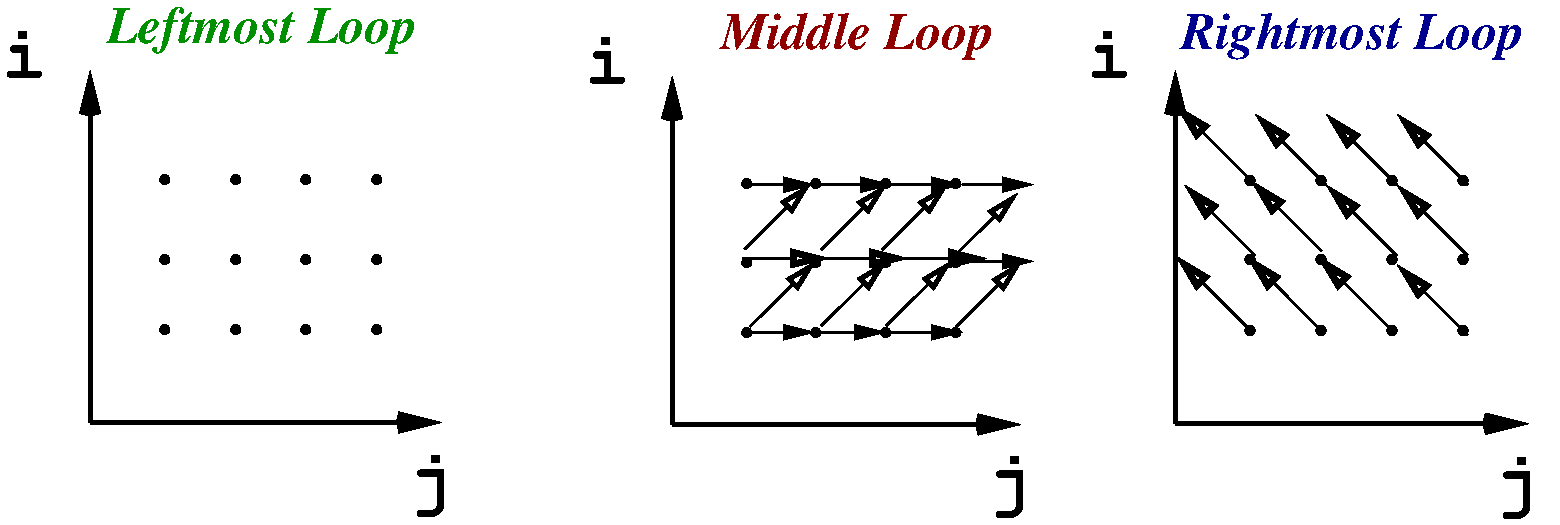
\includegraphics[height=23ex]{Figures/L5-LoopPar/LoopDeps}  

\alert{How can I summarize this information?} %Do I have to consider all cases?

\end{frame}





\begin{frame}[fragile,t]
  \frametitle{Aggregate Dependencies via Direction Vectors} % of CPU, Multicores, GPGPU

\begin{block}{Write the Direction Vectors for Each Loop:}
\begin{colorcode}
  DO i = 1, N            DO i = 2, N               DO i = 2, N
    DO j = 1, N            DO j = 2, N               DO j = 1, N 
S1    A[j,i]=A[j,i]..  S1   A[j,i]=A[j-1,i]...   S1    A[i,j]=A[i-1,j+1]...
    ENDDO              S2   B[j,i]=B[j-1,i-1]...     ENDDO
  ENDDO                  ENDDO ENDDO               ENDDO
\end{colorcode}
\end{block} 



\smallskip

Dependencies depicted via an edge {\em from} the stmt that executes first
in the loop nest, i.e., {\em the source}, {\em to} the one that executes later, {\em the sink}.

\smallskip

{\bf Def. Dependence Direction:} Assume $\exists$ a dependence from $S1$ in iteration $\vec{k}$
to $S2$ in $\vec{l}$ ($\vec{k}\leq\vec{l}$). 
\emp{\em Dependence-direction vector $\vec{D}(\vec{k},\vec{l})$}:
\begin{description}
    \item[1.] $\vec{D}(\vec{k},\vec{l})_m = $~``{\tt{}<}'' if $\vec{k}_m < \vec{l}_m$,
    \item[2.] $\vec{D}(\vec{k},\vec{l})_m = $~``{\tt{}=}'' if $\vec{k}_m = \vec{l}_m$,
    \item[3.] $\vec{D}(\vec{k},\vec{l})_m = $~``{\tt{}>}'' if $\vec{k}_m > \vec{l}_m$.
\end{description}

\medskip
If the source is a write and the sink a read then {\sc raw} dependency,\\iIf the source is a read then {\sc war}, if both are writes then {\sc waw}.  
\end{frame}


\begin{frame}[fragile,t]
  \frametitle{Parallelism and Loop Interchange} % of CPU, Multicores, GPGPU

\begin{block}{Direction Vectors/Matrix for Three Loops }
\begin{columns}
\column{0.27\textwidth}
\begin{colorcode}
  DO i = 1, N
    DO j = 1, N
S1    A[j,i]=A[j,i]..
    ENDDO
  ENDDO
For S1\mymath{\rightarrow}S1: 
    (j1,i1)=(j2,i2) 
    i1 \emp{=} i2 \& j1 \emp{=} j2

Direction matrix:
S1\mymath{\rightarrow}S1: \emp{[=,=]}
\end{colorcode}
\column{0.32\textwidth}
\begin{colorcode}
  DO i = 2, N
    DO j = 2, N
S1    A[j,i]=A[j-1,i]...
S2    B[j,i]=B[j-1,i-1]...
    ENDDO
  ENDDO
S1\mymath{\rightarrow}S1: (j1,i1)=(j2-1,i2)
        i1 \emp{=} i2 \& j1 \emp{<} j2
S2\mymath{\rightarrow}S2: (j1,i1)=(j2-1,i2-1)
        i1 \emp{<} i2 \& j1 \emp{<} j2
S1\mymath{\rightarrow}S1: \emp{[=,<]}
S2\mymath{\rightarrow}S2: \emp{[<,<]}
\end{colorcode}
\column{0.32\textwidth}
\begin{colorcode}
  DO i = 2, N
    DO j = 1, N
S1    A[i,j]=A[i-1,j+1]...
    ENDDO
  ENDDO
For S1\mymath{\rightarrow}S1: 
    (i1,j1) = (i2-1,j2+1)
    i1 \emp{<} i2 \& j1 \emp{>} j2

Direction matrix:
S1\mymath{\rightarrow}S1: \emp{[<,>]}
\end{colorcode}
\end{columns}
\end{block} 

{\bf Th. Parallelism:} A loop in a loop nest is parallel {\em iff} all its directions
are either {\tt =} or there exists an outer loop whose corresp. direction is {\tt <}. 

\smallskip

\alert{A direction vector cannot have $>$ as the first non-= symbol},\\
as that would mean that I depend on something in the future. 
\end{frame}

\begin{frame}[fragile,t]
  \frametitle{Parallelism and Loop Interchange} % of CPU, Multicores, GPGPU

\begin{block}{Direction Vectors/Matrix for Three Loops }
\begin{columns}
\column{0.27\textwidth}
\begin{colorcode}
  DO i = 1, N
    DO j = 1, N
S1    A[j,i]=A[j,i]..
    ENDDO
  ENDDO
For S1\mymath{\rightarrow}S1: 
    (j1,i1)=(j2,i2) 
    i1 \emp{=} i2 \& j1 \emp{=} j2

Direction matrix:
S1\mymath{\rightarrow}S1: \emp{[=,=]}
\end{colorcode}
\column{0.32\textwidth}
\begin{colorcode}
  DO i = 2, N
    DO j = 2, N
S1    A[j,i]=A[j-1,i]...
S2    B[j,i]=B[j-1,i-1]...
    ENDDO
  ENDDO
S1\mymath{\rightarrow}S1: (j1,i1)=(j2-1,i2)
        i1 \emp{=} i2 \& j1 \emp{<} j2
S2\mymath{\rightarrow}S2: (j1,i1)=(j2-1,i2-1)
        i1 \emp{<} i2 \& j1 \emp{<} j2
S1\mymath{\rightarrow}S1: \emp{[=,<]}
S2\mymath{\rightarrow}S2: \emp{[<,<]}
\end{colorcode}
\column{0.32\textwidth}
\begin{colorcode}
  DO i = 2, N
    DO j = 1, N
S1    A[i,j]=A[i-1,j+1]...
    ENDDO
  ENDDO
For S1\mymath{\rightarrow}S1: 
    (i1,j1) = (i1-1,j2+1)
    i1 \emp{<} i2 \& j1 \emp{>} j2

Direction matrix:
S1\mymath{\rightarrow}S1: \emp{[<,>]}
\end{colorcode}
\end{columns}
\end{block} 

{\bf Th. Loop Interchange:} A column permutation of the loops in a loop nest 
is legal {\em iff} permuting the direction matrix in the same way {\em does NOT result}
in a {\tt >} direction as the leftmost non-{\tt{}=} direction in a row. 

\end{frame}


\begin{frame}[fragile,t]
  \frametitle{Parallelism and Loop Interchange} 

\begin{block}{Direction Vectors/Matrix for Three Loops }
\begin{colorcode}
  DO i = 1, N            DO i = 2, N               DO i = 2, N
    DO j = 1, N            DO j = 2, N               DO j = 1, N 
S1    A[j,i]=A[j,i]..  S1   A[j,i]=A[j-1,i]...   S1    A[i,j]=A[i-1,j+1]...
    ENDDO              S2   B[j,i]=B[j-1,i-1]...     ENDDO
  ENDDO                  ENDDO ENDDO               ENDDO

For S1\mymath{\rightarrow}S1: j1 = j2    For S1\mymath{\rightarrow}S1: j1 = j2-1          For S1\mymath{\rightarrow}S1: i1 = i2-1
            i1 = i2                i1 = i2                    j1 = j2+1
(i2,j2)-(i1,j1)=         (i2,j2)-(i1,j1)=\emp{[=,<]}        (i2,j2)-(i1,j1)=\emp{[<,>]}
\emp{[=,=]}                  For S2\mymath{\rightarrow}S2: j1 = j2-1
                                   i1 = i2-1
                         (i2,j2)-(i1,j1)=\emp{[<,<]}
\end{colorcode}
\end{block} 

Interchange is safe for the first and second nests, but not for the third!\\
e.g., \emp{\tt [=,<]}$~~~\rightarrow~~~$ \emph{\tt [<,=]}$~~~~~~~~~$(for the second loop nest)\\
$~~~~~~$\emp{\tt [<,<]}$~~~~~~~~~~~~$\emph{\tt [<,<]}

\pause\smallskip

After interchange, loop $j$ of the second loop nest is parallel.

\bigskip

\emph{\bf Corollary: A parallel loop can be always interchanged inwards.}
\end{frame}


\begin{frame}[fragile,t]
  \frametitle{Dependency Graph and Loop Distribution} 

{\bf Def. Dependency Graph:} edges from the source of the dependency, i.e., early iteration, 
to the sink, i.e., later iteration. 

\smallskip

{\bf Th. Loop Distribution:} Statements that are in a dependence cycle remain in one 
(sequential) loop.   The others are distributed to separate loops in graph order; 
if no cycle then parallel loops.\smallskip

\begin{block}{Vectorization Example: Remember Vector Machines?}
\begin{columns}
\column{0.34\textwidth}
\begin{colorcode}[fontsize=\scriptsize]
  DO i = 3, N
\emp{S1  A[i] = B[i-2] ...}
\alert{S2  B[i] = B[i-1] ...}
  ENDDO  

For S2\mymath{\rightarrow}S1: i1 = i2-2, \emp{[<]}
For S2\mymath{\rightarrow}S2: i1 = i2-1, \emp{[<]}
\end{colorcode}
\column{0.27\textwidth}\pause
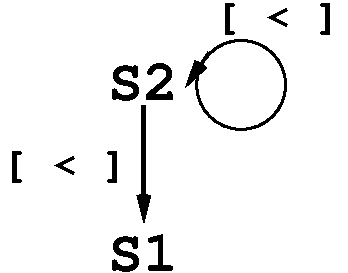
\includegraphics[height=12ex]{Figures/L5-LoopPar/LoopDistr}  
\column{0.30\textwidth}
\begin{colorcode}[fontsize=\scriptsize]
  \alert{DO} i = 3, N
S2  B[i] = B[i-1] ...
  \alert{ENDDO}

  \emphh{DOALL} i = 3, N
\emp{S1  A[i] = B[i-2] ...}
  \emphh{ENDDOALL}
\end{colorcode}
\end{columns}
\end{block}

\medskip

{\bf Corollary:} It is always legal to distribute a parallel loop;\\
\alert{but requires array expansion for local variables or if output
dependencies are present.}
\end{frame}

\begin{frame}[fragile,t]
  \frametitle{Loop Distribution May Require Array Expansion} 


\begin{columns}
\column{0.4\textwidth}
\begin{colorcode}[fontsize=\scriptsize]
  float tmp;
  for(i=2; i<N; i++) \{
    \emp{tmp} = 2*B[i-2]; 
    A[i] = tmp;
    B[i] = tmp+B[i-1]
  \}
\end{colorcode}
\column{0.53\textwidth}
\begin{colorcode}[fontsize=\scriptsize]
  \emph{float tmp[N]};
  for(int i=2; i<N; i++) \{
    tmp[i] = 2*B[i-2]; 
    B[i] = tmp[i]+B[i-1];
  \}

  \emph{forall(int i=2; i<N; i++)} \{
    A[i] = tmp[i];
  \}
\end{colorcode}
\end{columns}
\bigskip

No matter where {\tt tmp} is declared (inside or outside
the loop) it needs to be expanded into an array in order
to do loop distribution.\bigskip

If {\tt tmp} is declared outside the loop then requires \emp{\bf privatization}, \pause
because it actually causes frequent {\sc waw} dependencies.
However its value is written before being used within the same iteration.
Hence it is semantically equivalent to a locally declared variable,
which will remove the output ({\sc waw}) dependency.\bigskip

Distribution requires array expansion of the scalar {\tt tmp}.

\end{frame}


\begin{frame}[fragile,t]
  \frametitle{False Dependencies (WAR/WAW)} 

\begin{itemize}
    \item \emp{Cross-Iteration Anti Dependencies (WAR)} 
        correspond to a read from the array as it was 
        before the loop $\Rightarrow$ can be eliminated
        by reading from a copy of the array.\bigskip

    \item \emp{Cross-Iteration WAW Dependencies (WAW)}:\\
        If they correspond to the case in which every \emp{\bf read} from
        a scalar or array location is covered by a \emp{\bf previous same-iteration write}
        %a re-writing the same array elements
        %in different iterations 
        $\Rightarrow$ can be eliminated \emph{\bf privatization (renaming)},
        which semantically moves the declaration of the variable (scalar or array) 
        inside the loop.\bigskip

    \item Direction-vectors reasoning is limited to relatively
        simple loop nests, e.g., difficult to reason about 
        privatization in such a way.
\end  {itemize}
\end{frame}

\begin{frame}[fragile,t]
  \frametitle{False Dependencies (WAR/WAW)} 

\begin{block}{Anti Dependency (WAR) {\tt~~} and {\tt~~}Output Dependency (WAW)}
\begin{columns}
\column{0.40\textwidth}
\begin{colorcode}[fontsize=\scriptsize]
// \alert{OpenMP code:} 
// \alert{compile with g++ -fopenmp ...}
  float tmp = A[1];
  \emp{for (i=0; i<N-1; i++)}
\emp{S1  A[i] = A[i+1];} 
  A[N-1] = tmp;
//S1\mymath{\rightarrow}S1: i1+1=i2, \emp{[<]} WAR\pause

// Solution: copy A into A'
// and use A' for the reads!
float Acopy[N];
\#pragma omp parallel for
  \emph{for(i=0; i<N; i++)} \{
    Acopy[i] = A[i];
  \}
  tmp = A[1];
\emph{\#pragma omp parallel for} \emp{private(i)}
  for (i=0; i<N-1; i++) \{
    \emph{A[i] = Acopy[i+1];}
  \}
  A[N-1] = tmp;
\end{colorcode}

\column{0.55\textwidth}
\begin{colorcode}[fontsize=\scriptsize]
  int A[M];
  for(i=0; i<N; i++)\{
    for(int j=0, j<M; j++)
        \emp{A[j]} = (4*i+4*j) \% M;
    for(int k=0; k<N; k++)
        X[i,k]=X[i,k-1] * \emp{A[A[(2*i+k)\%M]]};
  \}

// \emp{The write to A[j] causes multiple WAWs},\pause
// \emph{but A is fully written in the inner loop} 
\emph{\#pragma omp parallel}\{
  int A[M];
\emph{\#pragma omp for}
  for(int i=0; i<N; i++)\{
    for(int j=0, j<M; j++)
        \emp{A[j]} = (4*i+4*j) \% M;
    for(int k=0; k<N; k++)
        X[i,k]=X[i,k-1] * \emp{A[A[(2*i+k)\%M]]};
  \}
\}
\end{colorcode}
\end{columns}
\end{block}

%free(A);

\end{frame}

\begin{frame}[fragile,t]
  \frametitle{Reduction is Typically Easy To Recognize} 

If all the statements in which a scalar variable {x} appears
are of the form {\tt x $\oplus$ = $exp$}, where {\tt x} does 
not appear in $\exp$ and $\oplus$ is associative 
then the cross-iteration RAWs on {\tt x} can be resolved by:
\begin{itemize}
    \item privatizing {\tt x} initialized with the neutral element,
    \item computing the per-processor partial values of {\tt x},
    \item reducing the {\tt x}s across processors and with the initial value.
\end  {itemize} 

\begin{columns}
\column{0.4\textwidth}
\begin{colorcode}[fontsize=\scriptsize]
// compilation requires g++ -fopenmp ...
  float x = 6.0;
\#pragma omp parallel for reduction(+:x) private(i,j)
  for(i=1; i<N; i++) \{
    for(j=1; j<N; j++) \{
      if ( A[i,j] >= 2.0 )    \emph{x += 2*A[i,j-1]};
      else if( A[i,j] > 0.0 ) \emph{x += A[i-1,j+1];}
    \}
    if (i \% (j+1) == 3) \emph{x += A[i,i];}
  \}
\end{colorcode}
\column{0.53\textwidth}

%\begin{colorcode}[fontsize=\scriptsize]
%// Semantically Equivalent to:
%  float x = 6.0;
%  float xs[NUM_THREADS];
%\#pragma omp parallel private(th_id)\{
%  th_id = omp_get_thread_num();
%\#pragma omp parallel for private(i,j)
%  for(i=0; i<N; i++) \{
%    for(j=0; j<N; j++) 
%      if ( A[i,j] >= 2.0 ) 
%        \emph{xs[th_id] += 2*A[i,j-1]*x};
%      else if( A[i,j] > 0.0 )
%        \emph{xs[th_id] += A[i,j+1]/x;}
%    if (i \% (j+1) == 3) 
%        \emph{xs[th_id] += A[i,i]}
%  \}
%\}
%x += reduce (+) 0.0 xs // Haskell-like code
%\end{colorcode}
\end{columns}
\end{frame}


\begin{frame}[fragile,t]
  \frametitle{Scan and Segmented Scan Are Difficult!} 

Compilers cannot recognize and parallelize even simple scans:
\begin{itemize}
    \item they raise a cross-iteration true dependency (RAW),
    \item they appear in a multitude of forms,
    \item hence they are difficult to analyze.
\end  {itemize} 

\begin{columns}
\column{0.4\textwidth}
\begin{colorcode}[fontsize=\scriptsize]
// What kind of scans are these?
1. A[0] = B[0];
   for(i=1; i<N; i++) \{
     A[i] = A[i-1] + B[i];
   \}
2. acc = 0;
   for(i=0; i<N; i++)\{
     acc = acc xor i;
     A[i] = acc;
   \}
3. for(j=0; j<M; j++) 
     A[0,j] = B[0,j];
   for(i=1; i<N; i++) \{
     for(j=0; j<M; j++)
       A[i,j] = A[i-1,j] + B[i,j];
   \}
\end{colorcode}
\column{0.53\textwidth}\pause
\begin{colorcode}[fontsize=\scriptsize]
1. let A = scanInc (+) 0 B

2. let A = scanInc (xor) 0 [0..N-1]

3. let A = scanInc (\mymath{\backslash} a b -> zipWith (+) a b) 
                   (replicate M 0.0) B \mymath{\equiv}
   let A = transpose \$ 
           map (scanInc (+) 0.0) \$
           transpose B 
             
\end{colorcode}
\end{columns}
\bigskip

\end{frame}

\section{Block Tiling: Matrix Multiplication Case Study}

\begin{frame}[fragile]
	\tableofcontents[currentsection]
\end{frame}

\begin{frame}[fragile,t]
  \frametitle{Matrix Multiplication: Loop Strip Mining} % of CPU, Multicores, GPGPU

\begin{columns}
\column{0.42\textwidth}
\begin{colorcode}[fontsize=\scriptsize]
DOALL i = 1, M, 1    \emphh{// Parallel}
  DOALL j = 1, N, 1  \emphh{// Parallel}
    float tmp = 0.0
    DO k = 1, U, 1 \emp{// Reduction}
      tmp += A[i,k]*B[k,j] 
    ENDDO                  
    C[i,j] = tmp;          
  ENDDO
ENDDO
\end{colorcode}
\column{0.55\textwidth}
$\leftarrow$Matrix Multiplication. Matrices:\smallskip
\begin{itemize}
    \item input {\tt A} has {\tt M} rows and {\tt U} columns
    \item input {\tt B} has {\tt U} rows and {\tt N} columns
    \item result {\tt C} has {\tt M} rows and {\tt N} columns 
\end{itemize}

Loops of indices {\tt i} and {\tt j} are parallel
(can be proved by direction vectors).
\end{columns}
\medskip

\emph{Accesses to {\tt A} and {\tt B} invariant to loops {\tt i} and {\tt j} $\Rightarrow$ Block Tiling to optimize locality of reference!}  
\pause
\bigskip

First step: Strip Mining, always safe since 
the transformed loop executes the same instructions in the same 
order as the original loop:\medskip

\begin{columns}
\column{0.47\textwidth}
\begin{colorcode}[fontsize=\scriptsize]
DO i = 1, N, 1  \alert{// stride 1}
  loop_body(i)
ENDDO


\end{colorcode}
\column{0.47\textwidth}
\begin{colorcode}[fontsize=\scriptsize]
DO ii = 1, N, T        \alert{// stride T}
  DO i = ii, MIN(ii+T-1,N), 1 
    loop_body(i)
  ENDDO
ENDDO
\end{colorcode}
\end{columns}
\end{frame}


\begin{frame}[fragile,t]
  \frametitle{Matrix Multiplication: Loop Interchange} % of CPU, Multicores, GPGPU

After strip mining all loops with a tile of size {\tt T}:
\begin{colorcode}[fontsize=\scriptsize]
\emp{DOALL ii = 1, M, T}
  \emph{DOALL i = ii, MIN(ii+T-1,M), 1}     \blue{// loop}
    \emp{DOALL jj = 1, N, T}               \blue{// interchange.} \alert{Why Safe?}
      \emph{DOALL j = jj, MIN(jj+T-1,N), 1}
        float tmp = 0.0
        DO kk = 1, U, T
          DO k = kk, MIN(kk+T-1,U), 1
            tmp += A[i,k]*B[k,j]
        ENDDO ENDDO
        C[i,j] = tmp;
ENDDO ENDDO ENDDO ENDDO
\end{colorcode}
\medskip
\pause

The second step is to apply loop interchange between the loops 
of indices {\tt i} and {\tt jj}. This is safe because loop {\tt i}
is parallel, hence it can always be interchanged inwards!

\end{frame}

\begin{frame}[fragile,t]
  \frametitle{Matrix Multiplication: Summarizing Read Subscripts} % of CPU, Multicores, GPGPU

After loop interchange we have a grid shape, as in CUDA:
\begin{colorcode}[fontsize=\scriptsize]
\emp{DOALL ii = 1, M, T}                    // \emp{grid.y}
  \emp{DOALL jj = 1, N, T}                  // \emp{grid.x}
    \emph{DOALL i = ii, MIN(ii+T-1,M), 1}    // \emph{block.y}
      \emph{DOALL j = jj, MIN(jj+T-1,N), 1}  // \emph{block.x}
        float tmp = 0.0
        DO kk = 1, U, T
          \blue{DO k = kk, MIN(kk+T-1,U), 1}
            \blue{tmp += A[i,k]*B[k,j]}
          \blue{ENDDO} 
        ENDDO
        C[i,j] = tmp;
ENDDO ENDDO ENDDO ENDDO
\end{colorcode}
\medskip

\blue{The third step is to summarize the subscripts of {\tt A} and {\tt B}
read inside the loop of index {\tt k}, for fixed {\tt ii}, {\tt jj} and {\tt kk}}
({\tt x:y} denotes {\tt [x$\ldots$y]}):\pause
\begin{itemize}
    \item {\tt A} subscripts \blue{\tt[ii~:~MIN(ii+T-1,M), kk~:~MIN(kk+T-1,U)]}
    \item {\tt B} subscripts \blue{\tt[kk~:~MIN(kk+T-1,U), jj~:~MIN(jj+T-1,N)]}
    \item Summaries have size at most {\tt T$^2$} \& independent on {\tt i}, 
            {\tt j}, and {\tt k} $\Rightarrow$ {\sc cuda}-block threads 
            cooperatively copy-in data to shared mem!   
\end  {itemize}

\end{frame}

\begin{frame}[fragile,t]
  \frametitle{Block Tiled Matrix Multiplication CUDA Kernel} % of CPU, Multicores, GPGPU

Shared memory padded with zeros to remove the branch from loop {\tt k}!  

\begin{columns}
\column{0.44\textwidth}
\begin{colorcode}[fontsize=\scriptsize]
\emp{DOALL ii = 1, M, T}   // \emp{grid.y}
  \emp{DOALL jj = 1, N, T} // \emp{grid.x}
    \emph{DOALL i = ii, MIN(ii+T-1,M), 1}    
      \emph{DOALL j = jj, MIN(jj+T-1,N), 1}
        float tmp = 0.0
        DO kk = 1, U, T
          \alert{//we would like to copy}
          \alert{//to shared memory here}
          \alert{//\& use it inside loop k}
          \blue{DO k = kk, MIN(kk+T-1,U), 1}
            \blue{tmp += A[i,k]*B[k,j]}
          \blue{ENDDO} 
        ENDDO
        C[i,j] = tmp;
ENDDO ENDDO ENDDO ENDDO
\end{colorcode}
\column{0.53\textwidth}\pause
\begin{colorcode}[fontsize=\scriptsize]
__global__ void matMultTiledKer( ... ) \{
  \alert{__shared__ T Ash[T][T], Bsh[T][T];}
  \emp{int ii = blockIdx.y * T;} //blockDim.x==T
  \emp{int jj = blockIdx.x * T;} //blockDim.y==T
  \emph{int tidy = threadIdx.y, i = tidy+ii;}
  \emph{int tidx = threadIdx.x, j = tidx+jj;}
  float tmp = 0.0;

  for(int kk=0; kk<U; kk+=T) \{
    \alert{Ash[tidy][tidx] = (i<M && kk+tidx<U) ?} 
                  \alert{A[i*U + (kk+tidx)] : 0.0;}
    \alert{Bsh[tidy][tidx] = (j<N && kk_tidy<U) ?} 
                  \alert{B[(kk+tidy)*N + j] : 0.0;}
    \blue{__syncthreads();}
    \blue{for(int k=0; k<T; k++) \{}
      \blue{tmp += Ash[tidy][k] * Bsh[k][tidx]}
    \blue{\} __syncthreads();}
  \} if (i<M && j<N) C[i*N + j] = tmp;
\}
\end{colorcode} 
\end{columns}


A global memory access amortized by (T-1) shared memory accesses.

\end{frame}

\begin{frame}[fragile,t]
  \frametitle{Measuring GFlops Performance} % of CPU, Multicores, GPGPU

Sequential matrix multiplication $\sim2\times M\times N\times U$
floating point operations. What is the GFlops performance of our implementation? 

\begin{columns}
\column{0.44\textwidth}
\begin{colorcode}[fontsize=\scriptsize]
// CPU code
int  dimy = ceil( ((float)M) / T ); 
int  dimx = ceil( ((float)N) / T );
dim3 block(T,T,1), grid(dimx,dimy,1);

unsigned long int elapsed;
struct timeval t_start,t_end,t_diff;
gettimeofday(&t_start, NULL); 
  // ignoring generic shared mem problems
  matMultTiledKer<T><<<grid, block>>>
            (d_A, d_B, d_C, U, M, N);

gettimeofday(&t_end, NULL);
timeval_subtract(&t_diff,
                 &t_end,&t_start);
elapsed=(t_diff.tv_sec*1e6 +
         t_diff.tv_usec); 
double flops = 2.0 * M * N * U; 
double gigaFlops=(flops*1.0e-3f) /
                 elapsed; 
\end{colorcode}
\column{0.53\textwidth}
\begin{colorcode}[fontsize=\scriptsize]
template <int T> // KERNEL
__global__ void matMultTiledKer( ... ) \{
  \alert{__shared__ float Ash[T][T], Bsh[T][T];}
  \emp{int ii = blockIdx.y * T;} //blockDim.x==T
  \emp{int jj = blockIdx.x * T;} //blockDim.y==T
  \emph{int tidy = threadIdx.y, i = tidy+ii;}
  \emph{int tidx = threadIdx.x, j = tidx+jj;}
  float tmp = 0.0;

  for(int kk=0; kk<U; kk+=T) \{
    \alert{Ash[tidy][tidx] = (i<M && kk+tidx<U) ?} 
                  \alert{A[i*U + (kk+tidx)] : 0.0;}
    \alert{Bsh[tidy][tidx] = (j<N && kk_tidy<U) ?} 
                  \alert{B[(kk+tidy)*N + j] : 0.0;}
    \blue{__syncthreads();}
    \blue{for(int k=0; k<T; k++) \{}
      \blue{tmp += Ash[tidy][k] * Bsh[k][tidx]}
    \blue{\} __syncthreads();}
  \} if (i<M && j<N) C[i*N + j] = tmp;
\}
\end{colorcode} 
\end{columns}

\end{frame}



\section{Coalesced Accesses: Matrix Transposition Case Study}

\begin{frame}[fragile]
	\tableofcontents[currentsection]
\end{frame}

\begin{frame}[fragile,t]
  \frametitle{Matrix Transposition: Motivation} 

\begin{columns}
\column{0.42\textwidth}
\begin{colorcode}[fontsize=\scriptsize]
// Non-Coalesced Memory Access
// Transposition to coalesce it \mymath{\Rightarrow}
DOALL i = 0 to N-1  // \emph{parallel}
  tmpB = A[i,0] * A[i,0]
  B[i,0] = tmpB
  DO j = 1, 63 // \emp{sequential}
    tmpA   = A[i, j]
    accum  = tmpB*tmpB + tmpA*tmpA
    B[i,j] = accum
    tmpB   = accum
  ENDDO
ENDDO
\end{colorcode}
\column{0.55\textwidth}
\begin{colorcode}[fontsize=\scriptsize]
A' = transpose(A)
DOALL i = 0 to N-1  // \emph{parallel}
  tmpB = A'[0,i] * A'[0,i]
  B'[0,i] = tmpB
  DO j = 1, 63 // \emp{sequential}
    tmpA   = A'[j, i]
    accum  = tmpB*tmpB + tmpA*tmpA
    B'[j, i] = accum
    tmpB     = accum
  ENDDO
ENDDO
B = transpose(B')
\end{colorcode}
\end{columns}
\bigskip

\emp{The transformed program performs about twice the number of
accesses to global memory than the original.}  
\medskip

\emph{But exhibits only coalesced accesses!}\\
\textbf{Coalesced Access:} a (half) warp accesses in a {\sc simd} instruction consecutive memory (word) locations. 
\medskip

\alert{What else could we have done to achieve the same effect?}\\\pause
\emph{Loop Interchange. Does it works in general?}
\end{frame}


\begin{frame}[fragile,t]
  \frametitle{Transposition: Strip Mining, Interchange \& Kernel} 
\vspace{-1ex}
\begin{columns}
\column{0.42\textwidth}
\begin{colorcode}[fontsize=\scriptsize]
//\emphh{Both loops are parallel}
//Strip mining \& interchange\mymath{\Rightarrow}
for(i = 0; i < rowsA; i++) \{    
  for(j = 0; j < colsA; j++) \{ 
    trA[j*rowsA+i] = A[i*colsA+j];
\} \}
\end{colorcode}
\column{0.55\textwidth}
\begin{colorcode}[fontsize=\scriptsize]
\emp{for(ii=0; ii<rowsA; ii+=T) \{}
  \emp{for(jj=0; jj<colsA; jj+=T) \{}
    \emphh{for(i=ii; i<min(ii+T,rowsA); i++) \{}
      \emphh{for(j=jj; j<min(jj+T,colsA); j++) \{}
        \blue{trA[j*rowsA+i]} = A[i*colsA+j];
\} \} \} \}
\end{colorcode}
\end{columns}

\pause

\begin{columns}
\column{0.5\textwidth}
\begin{colorcode}[fontsize=\scriptsize]
__global__ void matTranspose(
        float* A,  float* trA, 
        int rowsA, int colsA  ) \{
  __shared__ float tile[T][\alert{T}+1];
  int tidx = threadIdx.x;
  int tidy = threadIdx.y;
  int j    = blockIdx.x*T + tidx;
  int i    = blockIdx.y*T + tidy;
  if( j < colsA && i < rowsA )
    tile[tidy][tidx] = A[i*colsA+j];
  __syncthreads();
  \blue{i = blockIdx.y*T + threadIdx.x;} 
  \blue{j = blockIdx.x*T + threadIdx.y;}
  \blue{if( j < colsA && i < rowsA )}
    \blue{trA[j*rowsA+i] = tile[tidx]\alert{[tidy]};}
\}
\end{colorcode}
\column{0.47\textwidth}
\begin{itemize}
    \item \blue{Trick is to write the element of the symmetric thread in the same block.}
    \item \alert{What is the problem?}\pause
    \item Number of shared memory banks typically 16 or 32.
    \item T is also either 16 or 32 $\Rightarrow$
    \item 16 consecutive threads will read the same 
            memory bank at the same time.
    \item \emph{Solution: {\tt tile[T][\alert{T+1}];} }
\end  {itemize}
\end{columns}

\end{frame}


\begin{frame}[fragile,t]
  \frametitle{Lessons Learned So Far} 

\begin{itemize}
    \item Tiled transposition is less that $3\times$ faster
            than the naive version,
    \item but the motivating example runs much faster that that %(on some machines $8\times$)
            when transposition coalesces accesses to arrays 
            {\tt A} and {\tt B}. \alert{Why?}\pause
    \item \emp{Better to eliminate rather than hide latency.}
            Impact of hardware multi-threading limited  
            by the amount of available resources!\bigskip

    \item Generic Array of Tuples using shared memory:\pause requires a class
            with a ``volatile'' assignment operator. [Esben Skaarup]. 
    \item I believe it is safe to ignore the warnings; they can be
            eliminated at the expense of writing awkward code.\bigskip

    \item Shared-memory of generic type [Aske Dorge]:\pause
            empirically, $\sim8$ words of shared memory per 
            thread does not degrade perform.
    \item Simple solution: declare in kernel a shared memory
            array of type {\tt char}, then cast it to the generic type. 
            Set the size when calling the kernel to {\tt block\_size*32} bytes.
\end  {itemize}

\end{frame}


\begin{frame}[fragile,t]
  \frametitle{Constant (Read-Only) Memory in CUDA} 

\begin{itemize}
    \item 64KB of {\tt \_\_constant\_\_} memory on device (global/slow), 
            cached in each multiprocessor, e.g., 8KB (fast).\smallskip
    \item May reduce the required memory bandwidth:
            \begin{itemize}
                \item if found in cache, then no extra traffic,
                \item if a (half) warp accesses the same location and 
                        misses in cache $\Rightarrow$
                        only one request is sent and the result is
                        broadcast back to all,
                \item \alert{serialized} accesses if a warp of threads
                        read different locations!
                \item latency can range from one to hundreds of cycles.
            \end{itemize}\smallskip
    \item \emph{Best Use: when an entire block accesses 
                the same location in the same SIMD instruction}:
            even on a miss, the first warp brings the data in cache @ minimal traffic,
            the rest find it in cache. 
\end  {itemize}

\begin{columns}
\column{0.4\textwidth}
\begin{colorcode}[fontsize=\scriptsize]
// \emphh{C in __constant__ memory: Good!}
DO i = 1, N, 1   \emp{// grid}
  DO j = 1, M, 1 \emp{// block(s)}
    A[i,j] = A[i,j] \% C[i]
ENDDO
\end{colorcode}
\column{0.55\textwidth}
\begin{colorcode}[fontsize=\scriptsize]
// \alert{C in __constant__ memory: Bad!}
DO i = 1, N, 1   \emp{// grid}
  DO j = 1, M, 1 \emp{// block(s)}
    A[i,j] = A[i,j] \% C[j]
ENDDO
// \emphh{Either global memory or loop interchange}
\end{colorcode}
\end{columns}
\end{frame}


\section{Non-Trivial Synchronization: Histogram Case Study}
\begin{frame}[fragile]
	\tableofcontents[currentsection]
\end{frame}

\begin{frame}[fragile,t]
  \frametitle{Histogram: Problem Statement}
  
\begin{block}{Sequential Pseudocode \mbox{~~~~~~}\&\mbox{~~~~~~} Notation/Parameters:}
\begin{columns}
\column{0.4\textwidth}
\begin{colorcode}[fontsize=\scriptsize]
for(int i = 0; i < N; i++ ) \{
    (ind, val) = fun(image,i);
    H[ ind ] += val;
\}
\end{colorcode}
\column{0.54\textwidth}
\begin{colorcode}[fontsize=\scriptsize]
H = histogram
B = sizeof(H), e.g., 4\mymath{\times}4 \mymath{\dots} 64\mymath{\times}64 
N = sizeof(image), e.g., 256\mymath{\times}256\mymath{\times}256 
P = degree of parallelism (\# of cores)
\end{colorcode}
\end{columns}
\end{block} 

\bigskip
Typically, the additions to a histogram are {\tt 1},
but in this case two locations of the histogram are
incremented with {\tt val} and {\tt 1.0-val} (not shown).\bigskip  

{\tt ind} values are unstructured and may generate data races\\
if loop iterations are executed out of order, i.e., in parallel.

%\pause
\bigskip
However the code looks like a reduction on arrays $\Rightarrow$ can be \emph{parallelized}.

%\begin{center} 
%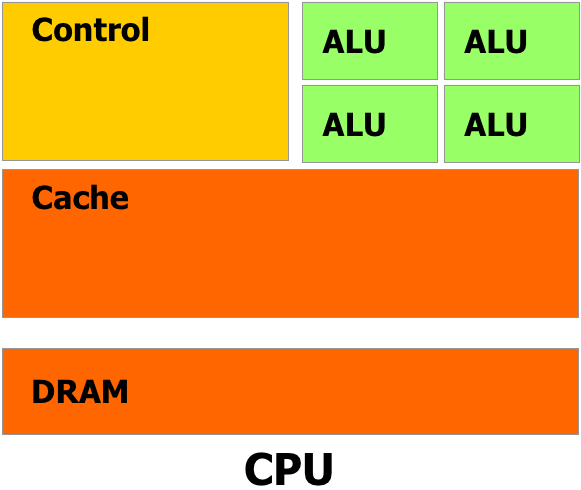
\includegraphics[height=20ex]{figures/MulticoreArch.png}  
%$\mbox{ }\mbox{ }\mbox{ }\mbox{ }\mbox{ }\mbox{ }\mbox{ }\mbox{ }\mbox{ }\mbox{ }\mbox{ }\mbox{ }\mbox{ }\mbox{ }\mbox{ }\mbox{ }$ 
%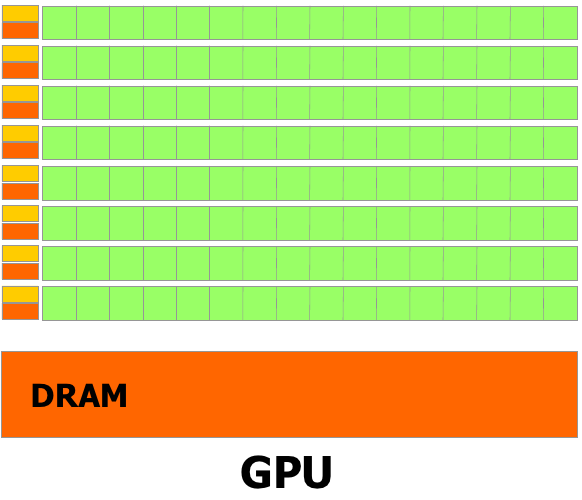
\includegraphics[height=20ex]{figures/GPGPUarch.png}  
%\end{center} 
\end{frame}


\begin{frame}[fragile,t]
  \frametitle{Histogram: OpenMP Code}
  
\begin{block}{ One Histogram/Thread \mbox{~~~~~~} \& \mbox{~~~~~~} Reduce Across Histograms }
\begin{columns}
\column{0.48\textwidth}
\begin{colorcode}[fontsize=\scriptsize]
int   P  = omp_get_num_threads(); 
REAL* pH = new REAL[P*B]; 
\emph{#pragma omp parallel}
\{ int   th_id = omp_get_thread_num();
  REAL* privH = pH + th_id * B;
  for(int i=0; i<B; i++) privH[i]=0.0;

\emph{#pragma omp for schedule(static)}
  \emp{for( int i=0; i < N; i++ )} \{
    (ind, val) = fun(image,i);
    privH[ ind ] += val;
  \} // \emp{end par for}
\end{colorcode}
\column{0.48\textwidth}
\begin{colorcode}[fontsize=\scriptsize]
// Assuming B big enough
pH' = parallel_transpose(pH);

\emph{#pragma omp for schedule(static)}
  \emp{for( int i=0; i<B; i++ )} \{
     for( int p=0; p<P; p++ ) \{
       H[i] += pH'[i*P + p];
     \}
  \} // \emp{end par for}
\} // \emp{end OMP parallel region}
\end{colorcode}
\end{columns}
\end{block} 

\bigskip

Work Efficient: $O({\tt P} \times {\tt B}) \leq O({\tt N})$.
Typically only the outer loop of the (image) nest is executed in parallel,
since {\tt P} is relatively small. 

\bigskip

The alternative is to not privatize \& reduce, but instead to 
provide lock-free (fine-grain) synchronization for each index 
in the histogram. 


\end{frame}


\begin{frame}[fragile,t]
  \frametitle{What Is Different for GPGPU Parallelization ?}
  
Differences:
\begin{itemize}
    \item Quite a few more cores, hence need to exploit all levels of parallelism,\bigskip %\pause \bigskip
    \item No (illusion of) constant-time random-memory access, e.g.,
            global memory accesses are up to two order of magnitude 
            more expensive than (scarce) local memory,\bigskip
    \item Synchronization primitives limited to local workgroup, i.e., barriers, 
            and can simulate {\sc cas}-like instructions at warp level. 
\end{itemize}

%\pause
%\bigskip

\end{frame}


\begin{frame}[fragile,t]
  \frametitle{Intuition}
  
\begin{itemize}
    \item If possible, keep histograms in local memory, 
            e.g., about $16$ ``local'' floats per thread:\bigskip
    \item If {\tt B} $\leq 16$ then $1$ histogram is maintained per thread,
    \item if {\tt B} $= 32$ then two threads build one histogram,
            using compare-and-swap {\sc cas} like locking.\bigskip
    \item In general if $16 <${\tt B} $\leq 32*8 = 512$ then up to $32$ (warp size)
            threads cooperate at building a histogram.\bigskip
    \item If {\tt B}$<=1024*8$ one CUDA block can cooperate at building
            a histogram -- must use CUDA atomic update instructions.\bigskip
    \item \emp{Difficulty:} for {\tt B}$\geq 1024*8$ need to keep the 
            histogram in global memory: prohibitively expensive
            due to irregular accesses.
\end{itemize}   


For simplicity use fix $L = 128$ the size of the CUDA block,
$G = 512$ the number of CUDA blocks, and unroll the loop: $N / (L\times G)$.
Work Efficient $\sim$ {\tt B} $ \leq $ {\tt N} / {\tt G}.
  
\end{frame}


\begin{frame}[fragile,t]
  \frametitle{ When {\tt L / WARP} Histograms Fit in Shared Memory }

\begin{block}{ CUDA Pseudocode; {\tt }, {\tt C} is the number of cooperating threads}
\begin{colorcode}[fontsize=\scriptsize]
\emph{__shared__ REAL sh_hist[ 16 * L ];} // L is the size of the block.
int i, tid = threadIdx.x;
// \emp{init local histogram(s)}
for( i = tid; i < 16*L; i += L ) sh_hist[ i ] = 0.0;  
__syncthreads();

// \emp{2) each thread executes U iterations sequentially.}
u = blockIdx.x * U * L + tid; 
for( i = u; i < u+(U*L); i += L ) \{
    (ind, val) = fun(image,i);

    \alert{ind = B * (tid/C) + ind;}  
    if ( C > 1 )
         \emph{raw_cas_update( sh_hist, ind, val );}
    else \emph{sh_hist[ ind ] += val;}
\}  __syncthreads();

// \emp{3) reduce locally across histograms}
\alert{for (i = 1; i < L/C && tid < B; i++)}
  \alert{sh_hist[tid] += sh_hist[tid + i*B]}
// \emp{4) commit the resulted local histogram to global storage } ...
\end{colorcode}
\end{block} 
%jhist += get_group_id(0) * B;
%for(t = TH_ID; t < B; t += L ) 
%    ghist[ t ] = sh_hist[ t ];   
\end{frame}


\begin{frame}[fragile,t]
  \frametitle{ When {\tt L / WARP} Histograms Fit in Shared Memory }

\begin{block}{ CUDA Pseudocode; {\tt }, {\tt C} is the number of cooperating threads}
\begin{colorcode}[fontsize=\scriptsize]
\emph{__shared__ REAL sh_hist[ 16 * L ];} // L is the size of the block.
int i, tid = threadIdx.x; 
// \emp{init local histogram(s)}
for( i = tid; i < 16*L; i += L ) sh_hist[ i ] = 0.0;  
__syncthreads();

// \emp{2) each thread executes U iterations sequentially.}
u = blockIdx.x * U * L + tid; 
for( i = u; i < u+(U*L); i += L ) \{
    (ind, val) = fun(image,i);
    \emphh{// we work with the transposed sh_hist}
    \emphh{ind = ( ind * L / C ) + ( tid / C );}  
    if ( C > 1 )
         \emph{raw_cas_update( sh_hist, ind, val );}
    else \emph{sh_hist[ ind ] += val;}
\}  __syncthreads();

// \emp{3) reduce locally across histograms}
\emphh{segm_scan_reg_block( sh_hist, B * L / C, L / C );}
// \emp{4) commit the resulted local histogram to global storage } ...
\end{colorcode}
\end{block} 
%jhist += get_group_id(0) * B;
%for(t = TH_ID; t < B; t += L ) 
%    ghist[ t ] = sh_hist[ t ];   
\end{frame}


\begin{frame}[fragile,t]
  \frametitle{ CAS-like Synchronization }

\begin{block}{ Function {\tt raw\_cas\_update} }
\begin{colorcode}[fontsize=\scriptsize]
void raw_cas_update(volatile REAL* sh_hist, ulong ind, REAL val) \{
    REAL acc, id  = (REAL)threadIdx.x;
    if (val == 0.0) return;
    bool repeat = true;
    while(repeat) \{
        acc = sh_hist[ind];
        \emp{sh_hist[ind] = id;} 
        \emp{if( sh_hist[ ind ] == id )} \{
            \emph{sh_hist[ ind ] = acc + val;}
            repeat = false;
        \}
    \}
\}
\end{colorcode}
\end{block} 

\bigskip

Bug in {\sc nvidia} implem of \textsc{OpenCL}: 
if barriers are placed inside {\tt while} loop the
execution does not deadlocks but incorrect result!\bigskip

\alert{How Do Results Look Like?}

\end{frame}


\section{Known Recurrences: Tridiagonal Solver Case Study}
\begin{frame}[fragile]
	\tableofcontents[currentsection]
\end{frame}

\begin{frame}[fragile,t]
  \frametitle{TRIDAG Motivation}

\emp{\em Stochastic Volatility Calibration}: given a set of observed prices
of contracts, identify a model of such prices, as a function of volatility
(unknown), time and strikes (known), and some other (unobserved) parameters.
\bigskip 

Volatility is modeled as a system of continuous differential
equations and solved via Crank-Nicolson finite-difference method:
%Compute function $f(x,t)$, $f : \mathcal{S} \times [0, T] \rightarrow \mathbb{R}$, 
%which solves the second order partial differential equation:

\begin{equation}
\frac{\partial f}{\partial t}(x,t)\mbox{ }+\mbox{ }\mu(x,t)\frac{\partial f}{\partial x}(x,t)\mbox{ }+\mbox{ }
\frac{1}{2}\sigma(x,t)^{2}\frac{\partial^{2} f}{\partial x^{2}}(x,t)\mbox{ }-\mbox{ }
r(x,t)f(x,t) = 0
\end{equation}

\smallskip

with terminal condition $f(x, T) = F(x), x \in \mathcal{S}$, where $F$ is known.

\bigskip

\emp{It comes down to solving this equation for many instances of $\mu, \sigma, r$.}

\end{frame}

\begin{frame}[fragile,t]
  \frametitle{Explicit Finite Difference Approach}

\begin{itemize}
    \item $\Delta x = (x_{J}-x_{1})/J$, $\Delta t = (t_{N}-t_{1})/N$\smallskip
    \item Uses Parametrizations:
        \begin{itemize}
            \item $D_xf_{j,n} = \frac{f_{j+1,n}-f_{j-1,n}}{2\Delta x}$,
                  $D_x^2f_{j,n} = \frac{f_{j+1,n}-2f_{j,n}+f_{j-1,n}}{(\Delta x)^2}$
            \item \alert{$D_t^{-}f_{j,n} = \frac{f_{j,n} - f_{j,n-1}}{\Delta t}$} 
        \end  {itemize}\smallskip
    \item Using this discretization in the differential equation yields:\\
             $f_{j,n-1} = \alpha_{j,n}f_{j-1,n} + \beta_{j,n}f_{j,n} + \gamma_{j,n}f_{j+1,n}$\smallskip
    \item where $f_{j,N}$ are known $\forall j \in \{1\ldots J\}$ and 
             we aim to find $f_{j,1}, \forall j$.\smallskip
    \item Trivial Parallel Algorithm Depth $O(T)$, Work $O(JT)$\smallskip

    \item \alert{However, mathematical reasoning requires $N >> J$, i.e.,
            a very fine-grained time discretization $\Rightarrow$ deep depth!}
\end  {itemize}


\end{frame}

\begin{frame}[fragile,t]
  \frametitle{Implicit Finite Difference Approach}

\begin{itemize}
    \item $\Delta x = (x_{J}-x_{1})/J$, $\Delta t = (t_{N}-t_{1})/N$\smallskip
    \item Uses Parametrizations:
        \begin{itemize}
            \item $D_xf_{j,n} = \frac{f_{j+1,n}-f_{j-1,n}}{2\Delta x}$,
                  $D_x^2f_{j,n} = \frac{f_{j+1,n}-2f_{j,n}+f_{j-1,n}}{(\Delta x)^2}$
            \item \alert{$D_t^{+}f_{j,n} = \frac{f_{j,n+1} - f_{j,n}}{\Delta t}$}
        \end  {itemize}\smallskip
    \item Using this discretization in the differential equation yields:\\
             $f_{j,n+1} = a_{j,n}f_{j-1,n} + b_{j,n}f_{j,n} + c_{j,n}f_{j+1,n}$\smallskip
    \item where $f_{j,N}$ are known $\forall j \in \{1\ldots J\}$ and 
             we aim to find $f_{j,1}, \forall j$,\smallskip
    \item meaning that we know $f_{j,n+1}~\forall j$ and want to compute $f_{j,n}~\forall j$\smallskip
    \item \emp{Requires solving a tridiagonal system (TRIDAG) at every time step; non-trivial
            to parallelize!}

    \item \alert{However, mathematical reasoning requires $N \sim J$, i.e.,
            the depth is reduced and degree of parallelism increased.}
\end  {itemize}

\end{frame}


\begin{frame}[fragile,t]
  \frametitle{TRIDAG Problem Statement}

\begin{block}{Needed: Parallel Algorithm for Computing $X$:} 

Given $A$ and $D$, find $X$ such that \emp{$A * X = D$}, \\
       where $A \in \mathbb{M}^{n \times n}$ is \emph{tridiagonal}, and $X$ and $D$ vectors of size $n$.

\begin{colorcode}[fontsize=\scriptsize]
                   \emp{\mymath{A}                   *    \mymath{X}     =    \mymath{D}}
 | b\mymath{\myindx{0}}  c\mymath{\myindx{0}}  0   0    ............... 0 |   | x\mymath{\myindx{0}}   |   | d\mymath{\myindx{0}}   |
 | a\mymath{\myindx{0}}  b\mymath{\myindx{1}}  c\mymath{\myindx{1}}  0    ............... 0 |   | x\mymath{\myindx{1}}   |   | d\mymath{\myindx{1}}   |
 | 0   a\mymath{\myindx{1}}  b\mymath{\myindx{2}}  c\mymath{\myindx{2}}  0  ............. 0 |   | x\mymath{\myindx{2}}   |   | d\mymath{\myindx{2}}   |
 | .................................. | * | .... | = | .... |
 | 0    0  ...    0    a\mymath{\myindx{n-3}} b\mymath{\myindx{n-2}} c\mymath{\myindx{n-2}} |   | x\mymath{\myindx{n-2}} |   | d\mymath{\myindx{n-2}} |
 | 0    0  ...    0    0    a\mymath{\myindx{n-2}} b\mymath{\myindx{n-1}} |   | x\mymath{\myindx{n-1}} |   | d\mymath{\myindx{n-1}} |

\end{colorcode}
\end{block}

At every step in the time series/discretization (sequential), we know matrix {\tt A} and
vector {\tt D} and need to compute in parallel vector {\tt X}.

\end{frame}




\begin{frame}[fragile,t]
  \frametitle{High-Level Solution (Sequential and Parallel)}

\begin{block}{Problem is to Find $X$ = $[x_0, ..., x_{n-1}]^T$ such that:} 

\begin{colorcode}[fontsize=\scriptsize]
                   \emp{\mymath{A}                   *    \mymath{X}     =    \mymath{D}}

 | b\mymath{\myindx{0}}  c\mymath{\myindx{0}}  0   0    ............... 0 |   | x\mymath{\myindx{0}}   |   | d\mymath{\myindx{0}}   |
 | a\mymath{\myindx{0}}  b\mymath{\myindx{1}}  c\mymath{\myindx{1}}  0    ............... 0 |   | x\mymath{\myindx{1}}   |   | d\mymath{\myindx{1}}   |
 | 0   a\mymath{\myindx{1}}  b\mymath{\myindx{2}}  c\mymath{\myindx{2}}  0  ............. 0 |   | x\mymath{\myindx{2}}   |   | d\mymath{\myindx{2}}   |
 | .................................. | * | .... | = | .... |
 | 0    0  ...    0    a\mymath{\myindx{n-3}} b\mymath{\myindx{n-2}} c\mymath{\myindx{n-2}} |   | x\mymath{\myindx{n-2}} |   | d\mymath{\myindx{n-2}} |
 | 0    0  ...    0    0    a\mymath{\myindx{n-2}} b\mymath{\myindx{n-1}} |   | x\mymath{\myindx{n-1}} |   | d\mymath{\myindx{n-1}} |

\end{colorcode}
\end{block}

\begin{itemize}
    \item STEP 1: Compute the LU decomposition of $A$, i.e., $A = L * U$, 
                  where $L$ and $U$ are lower and upper-diagonal matrices $\in \mathbb{M}^{n \times n}$. \bigskip
%
    \item STEP 2: Solve $L * Y = D$, i.e., compute partial solution $Y$. \bigskip
%
    \item STEP 3: Solve $U * X = Y$, i.e., compute problem solution $X$. \bigskip
%
    \item \emp{Each of the three steps needs to be parallel (of depth $O(log n)$)!}
\end{itemize}

\end{frame}



\begin{frame}[fragile,t]
  \frametitle{High-Level Solution (Sequential and Parallel)}

\begin{block}{Problem is to Find $X$ = $[x_0, ..., x_{n-1}]^T$ such that:} 

\begin{colorcode}[fontsize=\scriptsize]
                   \emp{\mymath{A}                   *    \mymath{X}     =    \mymath{D}}

 | b\mymath{\myindx{0}}  c\mymath{\myindx{0}}  0   0    ............... 0 |   | x\mymath{\myindx{0}}   |   | d\mymath{\myindx{0}}   |
 | a\mymath{\myindx{0}}  b\mymath{\myindx{1}}  c\mymath{\myindx{1}}  0    ............... 0 |   | x\mymath{\myindx{1}}   |   | d\mymath{\myindx{1}}   |
 | 0   a\mymath{\myindx{1}}  b\mymath{\myindx{2}}  c\mymath{\myindx{2}}  0  ............. 0 |   | x\mymath{\myindx{2}}   |   | d\mymath{\myindx{2}}   |
 | .................................. | * | .... | = | .... |
 | 0    0  ...    0    a\mymath{\myindx{n-3}} b\mymath{\myindx{n-2}} c\mymath{\myindx{n-2}} |   | x\mymath{\myindx{n-2}} |   | d\mymath{\myindx{n-2}} |
 | 0    0  ...    0    0    a\mymath{\myindx{n-2}} b\mymath{\myindx{n-1}} |   | x\mymath{\myindx{n-1}} |   | d\mymath{\myindx{n-1}} |
\end{colorcode}
\end{block}

\begin{colorcode}[fontsize=\scriptsize]
void tridag( REAL* a, REAL* b, REAL* c, REAL* d, int n, REAL* y, REAL* u )\{
    double beta;
    y[0] = d[0];   u[0] = b[0];
    for(int i=1; i<n; i++) \{     // distribute with
        beta = a[i] / u[i-1];     // direction vcts!
        u[i] = b[i] - beta*c[i-1];
        y[i] = d[i] - beta*y[i-1];
    \}
    y[n-1] = y[n-1]/u[n-1];
    for(int i=n-2; i>=0; i--) \{
        y[i] = (y[i] - c[i]*y[i+1]) / u[i];
\}  \}
\end{colorcode}

\end{frame}



\begin{frame}[fragile,t]
  \frametitle{LU-Decomposition Recurrences}

\begin{block}{Writing the LU decomposition: $A = L * U$, where $L, U \in \mathbb{M}^{n\times n}$} 
\begin{colorcode}[fontsize=\scriptsize]
            \mymath{A}                =           \mymath{L}           *          \mymath{U}
 
 | b\mymath{\myindx{0}}  c\mymath{\myindx{0}}  0   0  ... 0    |   | 1   0  0 ...   0 |   | u\mymath{\myindx{0}}  c\mymath{\myindx{0}}  0 ... 0    |
 | a\mymath{\myindx{0}}  b\mymath{\myindx{1}}  c\mymath{\myindx{1}}  0  ... 0    |   | m\mymath{\myindx{0}}  1  0 ...   0 |   | 0   u\mymath{\myindx{1}}  c\mymath{\myindx{1}}... 0    |
 | .................. c\mymath{\myindx{n-2}} | = | ................ | * | ....... u\mymath{\myindx{n-2}} c\mymath{\myindx{n-2}} |
 | 0   0 ...  0  a\mymath{\myindx{n-2}} b\mymath{\myindx{n-1}} |   | 0 ...  0  m\mymath{\myindx{n-2}} 1 |   | 0 ..... 0    u\mymath{\myindx{n-1}} |
\end{colorcode}
\end{block}

\bigskip

\begin{block}{LU-decomposition Recurrences:} 
\begin{colorcode}[fontsize=\scriptsize]
I.  First, compute {\tt u}\mymath{\myindx{i}, i \in \{0 .. n-1\}}: 
        I.a) {\tt u}\mymath{\myindx{0}} = {\tt b}\mymath{\myindx{0}}
        I.b) {\tt u}\mymath{\myindx{i}} = {\tt b}\mymath{\myindx{i}} - ( {\tt a}\mymath{\myindx{i-1}} * {\tt c}\mymath{\myindx{i-1}} ) / {\tt u}\mymath{\myindx{i-1}},   \mymath{i \in \{1 .. n-1\}}

II. Knowing the {\tt u}'s, we can easily compute the {\tt m}'s:
             {\tt m}\mymath{\myindx{i}} = {\tt a}\mymath{\myindx{i}} / {\tt u}\mymath{\myindx{i}}, \mymath{i \in \{0 .. n-2\}}
\end{colorcode}
\end{block}

%Testing to see the font here!

\end{frame}


\begin{frame}[fragile,t]
  \frametitle{The Difficult Recurrence of LU-Decomposition I.b) }

\begin{block}{ Parallel Algorithm: {\bf scan} with $\mathbb{M}^{2\times 2}$ multiplication operator} 
\begin{colorcode}[fontsize=\scriptsize]
Recurrence:
    I.a) {\tt u}\mymath{\myindx{0}} = {\tt b}\mymath{\myindx{0}}
    I.b) {\tt u}\mymath{\myindx{i}} = {\tt b}\mymath{\myindx{i}} - ( {\tt a}\mymath{\myindx{i-1}} * {\tt c}\mymath{\myindx{i-1}} ) / {\tt u}\mymath{\myindx{i-1}},  \mymath{i \in \{1 .. n-1\}} 

1) Substitute in I.b) {\tt u}\mymath{\myindx{i}\mbox{ }\leftarrow} {\tt q}\mymath{\myindx{i+1}} / {\tt q}\mymath{\myindx{i}}, 
        where q\mymath{\myindx{1}} = b\mymath{\myindx{0}} and q\mymath{\myindx{0}} = 1.0, i.e., u\mymath{\myindx{0}} == b\mymath{\myindx{0}} still holds! \emph{We obtain:}
    I.c) | q\mymath{\myindx{i+1}} | = | b\mymath{\myindx{i}}      - a\mymath{\myindx{i-1}} * c\mymath{\myindx{i-1}} | * | q\mymath{\myindx{i}}   |    
         | q\mymath{\myindx{i}}   |   | 1.0     0.0          |   | q\mymath{\myindx{i-1}} |    \mymath{i \in \{1 .. n-1\}}

2) Denoting the above \mymath{2\times 2} matrix by S\mymath{\myindx{i}\mbox{ }\in\mbox{ }\mathbb{M}\myindu{2\times{}2}} we obtain by induction:
    I.d) | q\mymath{\myindx{i+1}}  q\mymath{\myindx{i}} |\mymath{\myindu{T}} = ( S\mymath{\myindx{i}} * S\mymath{\myindx{i-1}} * S\mymath{\myindx{1}} ) * | b\mymath{\myindx{0}} 1.0 |\mymath{\myindu{T}}

3) We can compute all such matrices, i.e., S\mymath{\myindx{i}} * S\mymath{\myindx{i-1}} * S\mymath{\myindx{1}} with \mymath{i\in\{1..n-1\}}, 
   by applying {\bf{}scanInc} with the (associative) matrix-multiplication operator (*)
    I.e) matrices = scanInc (*) [S\mymath{\myindx{n-1}}, S\mymath{\myindx{n-2}}, ..., S\mymath{\myindx{1}}]

4) Finally, we compute each [q\mymath{\myindx{i+1}}, q\mymath{\myindx{i}}]\mymath{\myindu{T}} by multiplying its corresponding 
   matrix with [b\mymath{\myindx{0}}, 1.0]\mymath{\myindu{T}}, and compute u\mymath{\myindx{i}} = {\tt q}\mymath{\myindx{i+1}} / {\tt q}\mymath{\myindx{i}}. \emph{Both are PARALLEL:}
    I.f) q_pairs = map (matVectMult (b\mymath{\myindx{0}}, 1.0)) matrices
    I.g) u       = map (\mymath{\backslash} (x,y) \mymath{\rightarrow} x/y) q_pairs
\end{colorcode}
\end{block}

% , which has the identity \mymath{2 \times 2} matrix as neutral element.


\end{frame}


%\begin{frame}[fragile,t]
%  \frametitle{Implementing The LU-Decomposition Recurrences}
%
%5) Recurrence II, i.e., {\tt m}\mymath{\myindx{i}} = {\tt a}\mymath{\myindx{i}} / {\tt u}\mymath{\myindx{i}}, \mymath{i \in \{0 .. n-2\}} is written in parallel as:
%    {\tt{}m = map (lambda(x,y) -> x/y) (zip a u)}
%
%\begin{block}{ Haskell Code for Parallel LU Decomposition:} 
%\begin{colorcode}[fontsize=\scriptsize]
%\emp{computeLU_us_par} :: (Fractional a, Ord a) => [a] -> [a] -> [a] -> [a] 
%\emp{computeLU_us_par} a b c = 
%    let matMult2by2 [a1, a2, a3, a4] [b1, b2, b3, b4] =
%            [ (b1*a1+b2*a3), (b1*a2+b2*a4), (b3*a1+b4*a3), (b3*a2+b4*a4) ]
%        matVectMult b0 [a1, a2, a3, a4] = (a1*b0 + a2) / (a3*b0 + a4)
%            
%        b0             = head b
%        abc            = zip3 a (tail b) c
%        matrices\_inp  = map (lambda (a,b,c)->[b, (- (a * c)), 1.0, 0.0]) abc 
%        matrices\_out  = \emph{scanl matMult2by2 [1.0, 0.0, 0.0, 1.0] matrices\_inp}
%    in map (matVectMult b0) matrices\_out
%
%\emp{computeLU_ms_par} :: (Fractional a, Ord a) => [a] -> [a] -> [a]
%\emp{computeLU_ms_par} a u = map (lambda(x,y) -> x/y) (zip a u)
%
%\emp{decompLU} :: (Fractional a, Ord a) => [a] -> [a] -> [a] -> ([a],[a]) 
%\emp{decompLU} a b c = (\emph{computeLU_us_par} a b c, \emph{computeLU_ms_par} a us)
%\end{colorcode}
%\end{block}
%
%\end{frame}


\begin{frame}[fragile,t]
  \frametitle{STEP 2 \& 3: Solving For/Backward Recurrences}

\begin{block}{ STEP 2: Parallel Algorithm for $L * Y = D$ (forward recurrence)} 
\begin{colorcode}[fontsize=\scriptsize]
1) By doing the arithmetics, it comes down to solving the recurrence:
    II.a) y\mymath{\myindx{0}} = d\mymath{\myindx{0}}
    II.b) y\mymath{\myindx{i}} = d\mymath{\myindx{i}} - m\mymath{\myindx{i-1}} * y\mymath{\myindx{i-1}},   \mymath{i \in {1 .. n-1}}

2) We shall use {\bf scanInc} with linear-function-composition operator:
      i)   Consider f\mymath{\myindx{1}}(x) = a\mymath{\myindx{1}} + b\mymath{\myindx{1}}*x and f\mymath{\myindx{2}}(x) = a\mymath{\myindx{2}} + b\mymath{\myindx{2}}*x
      ii)  (f\mymath{\myindx{1}\mbox{ }\diamond\mbox{ }}f\mymath{\myindx{2}}) (x) = (a\mymath{\myindx{2}}+b\mymath{\myindx{2}}*a\mymath{\myindx{1}}) + (b\mymath{\myindx{1}}*b\mymath{\myindx{2}})*x
      iii) We represent such a function f as a pair (a, b), and implement 
           function application via operator: apply x (a, b) = a + b*x

3) Representing f\mymath{\myindx{i}} = (d\mymath{\myindx{i}}, -m\mymath{\myindx{i-1}}), \mymath{i \in {1 .. n-1}}
      i)   It follows by induction that y\mymath{\myindx{i}} = ( f\mymath{\myindx{i}} \mymath{\diamond} f\mymath{\myindx{i-1}} \mymath{\diamond} ... \mymath{\diamond} f\mymath{\myindx{1}} ) (d\mymath{\myindx{0}})
      ii)  We do a {\bf scanInc} with \mymath{\diamond} and neutral element (0.0, 1.0):
                f_out = scanInc (\mymath{\diamond}) (0.0, 1.0) [f\mymath{\myindx{1}}, ..., f\mymath{\myindx{n-1}}]
      iii) Finally, apply the f_out's to d\mymath{\myindx{0}} to compute all y\mymath{\myindx{i}}, \mymath{i\in\{1 .. n-1\}}
                y = map (apply d\mymath{\myindx{0}}) f_out
\end{colorcode}
\end{block}
\smallskip
\emph{STEP 3: Solving $U * X = Y$ is similar to STEP 2 (but {\it backwards}):}

      \emph{III.a) {\tt x}$_{n-1}$ = {\tt y}$_{n-1}$/{\tt u}$_{n-1}$ $\mbox{ }\mbox{ }\mbox{ }$}
          \emph{b) {\tt x}$_i$ = {\tt y}$_i$/{\tt u}$_i$ - {\tt c}$_{i}*${\tt x}$_{i+1}/${\tt u}$_i$, $i \in \{n-2 .. 0\}$}
\end{frame}

%\begin{frame}[fragile,t]
%  \frametitle{Putting The Implementation Together}
%\begin{block}{ Haskell Code for For/Backward Recurrence and TRIDAG} 
%\begin{colorcode}[fontsize=\scriptsize]
%\emp{\mymath{\diamond}} :: (Fractional a, Ord a) => (a,a) -> (a,a) -> (a,a)
%(a_1, b_1) \emp{\mymath{\diamond}} (a_2, b_2) = (a_2 + b_2*a_1, b_2*b_1)
%
%\emp{forward_rec} :: (Fractional a, Ord a) => [a] -> [a] -> [a] 
%\emp{forward_rec} d m = let d0 = head d
%                      fs = \emph{scanl (\mymath{\diamond}) (0.0,1.0) (zip (tail d) (map (0.0 -) m))}
%                  in map (lambda(a,b) -> a + b*d0) fs
%
%\emp{backward_rec} :: (Fractional a, Ord a) => [a] -> [a] -> [a] -> [a]
%\emp{backward_rec} y u c = let yuc = reverse (zip3 y u (c ++ [0.0]) )
%                         (y_nm1, u_nm1, c_nm1) = head yuc
%                         fs_inp = map (lambda(y,u,c)->(y/u,-c/u)) (tail yuc)
%                         fs_out = \emph{scanl (\mymath{\diamond}) (0.0, 1.0) fs_inp}
%                         x_nm1 = y_nm1 / u_nm1
%                     in reverse (map (lambda(a,b) -> a + b*x_nm1) fs_out)
%
%\emp{tridag} :: (Fractional a, Ord a) => [a] -> [a] -> [a] -> [a] -> [a]
%\emp{tridag} a b c d = let (u, m) = \emph{decompLU} a b c
%                     y = \emph{forward_rec} d m
%                 in      \emph{backward_rec} y u c
%\end{colorcode}
%\end{block}
%
%\end{frame}


\section{Imperative Context: Summarization of Array Indexes}
\begin{frame}[fragile]
	\tableofcontents[currentsection]
\end{frame}


\begin{frame}[fragile,t]
  \frametitle{Interprocedural Summarization of Array Indexes}


\begin{block}{ Independence-Summary Simple Example } \vspace{-1ex}
\begin{columns} 
\column{0.35\textwidth} 
\begin{colorcode}[fontsize=\scriptsize]
DO i = 1, N
  A(\emp{i+100}) = ...
  IF (x > 0) THEN
    ... = A(\emp{i})
  ENDIF
ENDDO
\end{colorcode}
\column{0.55\textwidth} 
\begin{center} \hspace{-4ex}
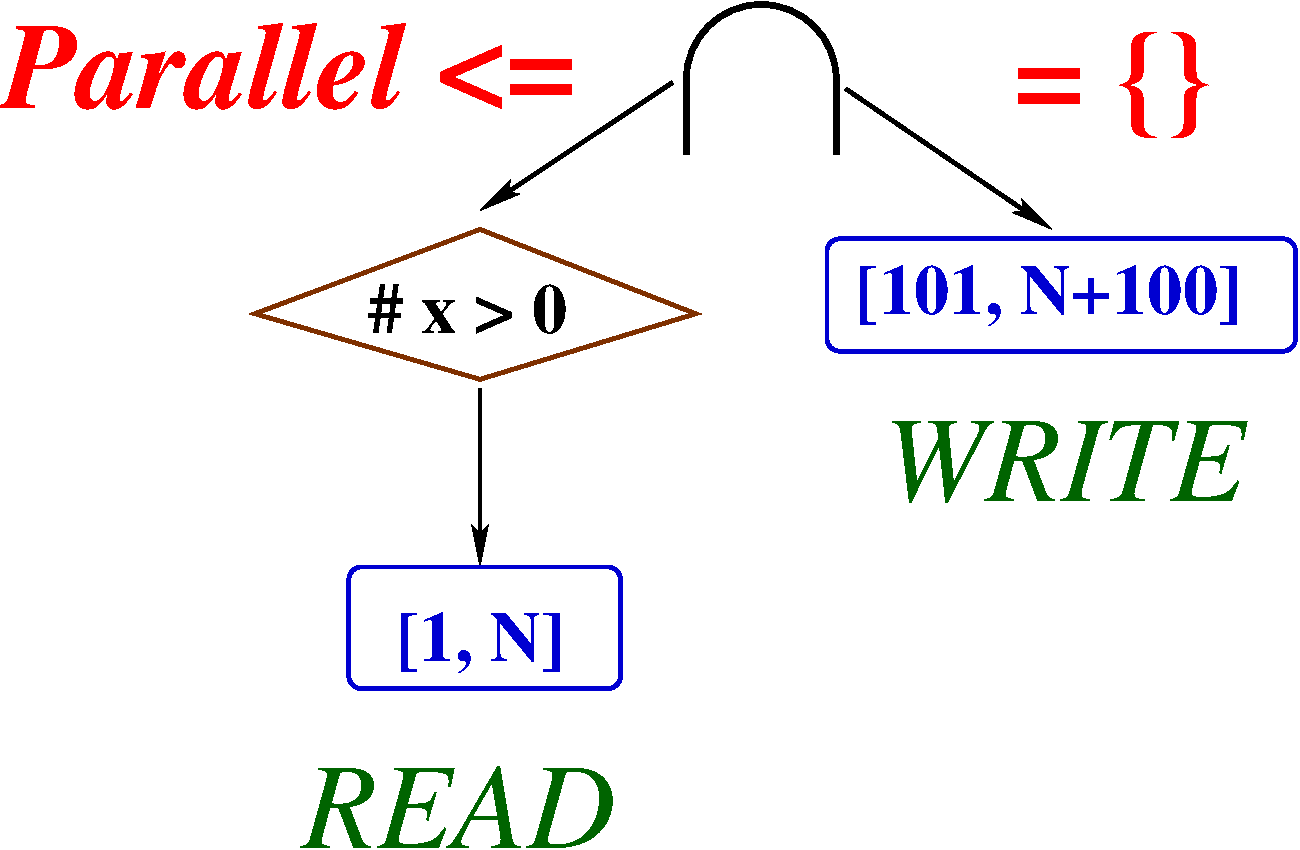
\includegraphics[height=15ex]{Figures/L5-LoopPar/SimpleInd}
\end{center}
\end{columns}
\end{block}


        \begin{itemize}
            \item Techniques that analyze read-write pairs of accesses become
                    very conservative on larger loops with non-trivial control flow.\smallskip   
            \item {\em Alternative:} inter-procedural summarization + model loop independence 
                    via an equation on summaries of shape $S = \emptyset$\\\smallskip 
            \item Decrease overhead by extracting lightweight predicates that prove 
                    independence at runtime, e.g., {\tt x~$\leq$~0~~$\vee$~~N~<~100}.
        \end{itemize} 

\bigskip

\alert{Show Calculix from \textsc{Spec2006}}!

\end{frame}


\begin{frame}[fragile,t]
  \frametitle{Building RO, RW, WF Summaries Interprocedurally}

Summaries ({\sc ro}, {\sc rw}, {\sc wf}) are
\begin{itemize}
    \item constructed via a bottom-up parse of the {\sc call} and {\sc cd} graphs,
    \item structural data-flow equations dictate how to compose consecutive regions,
            aggregate/translate across loops/callsites, ...
\end{itemize}

\pause

\begin{block}{Simplified {\tt solvh\_do20} from {\tt dyfesm}} \vspace{-1ex}
\begin{columns} 
\column{0.45\textwidth}
\begin{colorcode}[fontsize=\scriptsize]
\emp{DO i = 1, N}
    CALL geteu (XE(IA(i)), NP, SYM)
    CALL matmul(XE(IA(i)), NS)
\emp{ENDDO}

SUBROUTINE matmul(XE, NS)
  INTEGER NS, XE(*)
  DO j = 1, NS
    ...   = XE(j) ...
    XE(j) = ...
  ENDDO 
END
\end{colorcode}
\column{0.45\textwidth} 
\begin{colorcode}[fontsize=\scriptsize]
SUBROUTINE geteu(XE, NP, SYM)
  INTEGER NP, SYM, XE(16, *)
  
  IF (SYM .NE. 1) THEN
    DO i = 1, NP
      DO j = 1, 16
        XE(j, i) = ...
      ENDDO 
    ENDDO
  ENDIF
END
\end{colorcode}
\end{columns}
\end{block}

\end{frame}


%%%%%%%%%%%%%%%%%%%%%%%%%%%%%%
%%%%% SUBROUTINE getue
%%%%%%%%%%%%%%%%%%%%%%%%%%%%%%

\begin{frame}[fragile,t]
  \frametitle{Summarizing Subroutine {\tt geteu}}

\begin{block}{WF summary for {\tt geteu}; RO$_{geteu}$ $=$ RW$_{geteu}$ $= \emptyset$ } \vspace{-1ex}
\begin{columns} 
\column{0.45\textwidth} 
\begin{colorcode}[fontsize=\scriptsize]
\mymath{S\myindx{geteu}}  SUBROUTINE geteu(XE, NP, SYM)
         INTEGER NP, SYM, XE(16, *)  
\mymath{S\myindx{IF}}       \emph{IF (SYM .NE. 1) THEN}
\mymath{S\myindx{Li}}         \emp{DO i = 1, NP}
\mymath{S\myindx{Lj}}           \emp{DO j = 1, 16}
\mymath{S\myindx{WF}}             \alert{XE(j, i)} = ...
             \emp{ENDDO} 
           \emp{ENDDO}
         \emph{ENDIF}
       END
\end{colorcode}
\column{0.45\textwidth}
\begin{colorcode}[fontsize=\scriptsize]








\alert{\mymath{WF\myindu{XE}\myindx{S\myindx{WF}} = \{16*i+j-1\}}}
\end{colorcode}
\end{columns}
\end{block}


\begin{itemize}
    \item Loop Aggregation uses (intuitively) interval arithmetic: \smallskip
    \item Loop $i$: $\{16*i + j - 1 \mbox{ }\mbox{ }|\mbox{ } j \in \{1..\mbox{ }16\}\} \rightarrow \emp{16*i + [0,15]}$ \smallskip
    \item Loop $j$: $\{16*i + [0,15] \mbox{ }|\mbox{ } i \in \{1..NP\}\} \rightarrow \emp{[0, 16*NP-1]}$  \smallskip
    \item Branches introduce predicated nodes, e.g., \emph{$WF^{XE}_{S_{if}} = WF^{XE}_{S_{geteu}}$} 
\end{itemize}
\end{frame}

%%%%%%%%%%%%%%%%%%%%%%%%%%%%%%%%%%%%%%%%%%%%%%%%%%%%

\begin{frame}[fragile,t]
  \frametitle{Summarizing Subroutine {\tt geteu}}

\begin{block}{WF summary for {\tt geteu}; RO$_{geteu}$ $=$ RW$_{geteu}$ $= \emptyset$ } \vspace{-1ex}
\begin{columns} 
\column{0.45\textwidth} 
\begin{colorcode}[fontsize=\scriptsize]
\mymath{S\myindx{geteu}}  SUBROUTINE geteu(XE, NP, SYM)
         INTEGER NP, SYM, XE(16, *)  
\mymath{S\myindx{IF}}       \emph{IF (SYM .NE. 1) THEN}
\mymath{S\myindx{Li}}         \emp{DO i = 1, NP}
\mymath{S\myindx{Lj}}           \emp{DO j = 1, 16}
\mymath{S\myindx{WF}}             \alert{XE(j, i)} = ...
             \emp{ENDDO} 
           \emp{ENDDO}
         \emph{ENDIF}
       END
\end{colorcode}
\column{0.45\textwidth}
\begin{colorcode}[fontsize=\scriptsize]

\emp{\mymath{WF\myindu{XE}\myindx{S\myindx{Lj}} = 16*i + [0,15]}}

\alert{\mymath{WF\myindu{XE}\myindx{S\myindx{WF}} = \{16*i+j-1\}}}
\end{colorcode}
\end{columns}
\end{block}


\begin{itemize}
    \item Loop Aggregation uses (intuitively) interval arithmetic: \smallskip
    \item Loop $i$: $\{16*i + j - 1 \mbox{ }\mbox{ }|\mbox{ } j \in \{1..\mbox{ }16\}\} \rightarrow \emp{16*i + [0,15]}$ \smallskip
    \item Loop $j$: $\{16*i + [0,15] \mbox{ }|\mbox{ } i \in \{1..NP\}\} \rightarrow \emp{[0, 16*NP-1]}$  \smallskip
    \item Branches introduce predicated nodes, e.g., \emph{$WF^{XE}_{S_{if}} = WF^{XE}_{S_{geteu}}$} 
\end{itemize}
\end{frame}


%%%%%%%%%%%%%%%%%%%%%%%%%%%%%%%%%%%%%%%%%%%%%%%%%%%%

\begin{frame}[fragile,t]
  \frametitle{Summarizing Subroutine {\tt geteu}}

\begin{block}{WF summary for {\tt geteu}; RO$_{geteu}$ $=$ RW$_{geteu}$ $= \emptyset$ } \vspace{-1ex}
\begin{columns} 
\column{0.45\textwidth} 
\begin{colorcode}[fontsize=\scriptsize]
\mymath{S\myindx{geteu}}  SUBROUTINE geteu(XE, NP, SYM)
         INTEGER NP, SYM, XE(16, *)  
\mymath{S\myindx{IF}}       \emph{IF (SYM .NE. 1) THEN}
\mymath{S\myindx{Li}}         \emp{DO i = 1, NP}
\mymath{S\myindx{Lj}}           \emp{DO j = 1, 16}
\mymath{S\myindx{WF}}             \alert{XE(j, i)} = ...
             \emp{ENDDO} 
           \emp{ENDDO}
         \emph{ENDIF}
       END
\end{colorcode}
\column{0.45\textwidth}
\begin{colorcode}[fontsize=\scriptsize]




\emp{\mymath{WF\myindu{XE}\myindx{S\myindx{Li}} = [0,16*NP-1]}}

\emp{\mymath{WF\myindu{XE}\myindx{S\myindx{Lj}} = 16*i + [0,15]}}

\alert{\mymath{WF\myindu{XE}\myindx{S\myindx{WF}} = \{16*i+j-1\}}}
\end{colorcode}
\end{columns}
\end{block}


\begin{itemize}
    \item Loop Aggregation uses (intuitively) interval arithmetic: \smallskip
    \item Loop $i$: $\{16*i + j - 1 \mbox{ }\mbox{ }|\mbox{ } j \in \{1..\mbox{ }16\}\} \rightarrow \emp{16*i + [0,15]}$ \smallskip
    \item Loop $j$: $\{16*i + [0,15] \mbox{ }|\mbox{ } i \in \{1..NP\}\} \rightarrow \emp{[0, 16*NP-1]}$  \smallskip
    \item Branches introduce predicated nodes, e.g., \emph{$WF^{XE}_{S_{if}} = WF^{XE}_{S_{geteu}}$} 
\end{itemize}
\end{frame}


%%%%%%%%%%%%%%%%%%%%%%%%%%%%%%%%%%%%%%%%%%%%%%%%%%%%

\begin{frame}[fragile,t]
  \frametitle{Summarizing Subroutine {\tt geteu}}

\begin{block}{WF summary for {\tt geteu}; RO$_{geteu}$ $=$ RW$_{geteu}$ $= \emptyset$ } \vspace{-1ex}
\begin{columns} 
\column{0.45\textwidth} 
\begin{colorcode}[fontsize=\scriptsize]
\mymath{S\myindx{geteu}}  SUBROUTINE geteu(XE, NP, SYM)
         INTEGER NP, SYM, XE(16, *)  
\mymath{S\myindx{IF}}       \emph{IF (SYM .NE. 1) THEN}
\mymath{S\myindx{Li}}         \emp{DO i = 1, NP}
\mymath{S\myindx{Lj}}           \emp{DO j = 1, 16}
\mymath{S\myindx{WF}}             \alert{XE(j, i)} = ...
             \emp{ENDDO} 
           \emp{ENDDO}
         \emph{ENDIF}
       END
\end{colorcode}
\column{0.45\textwidth}
\begin{colorcode}[fontsize=\scriptsize]
          \emph{\mymath{(SYM \neq 1)}}
\emph{\mymath{WF\myindu{XE}\myindx{S\myindx{IF}} =}       \mymath{\downarrow}}
          \emph{\mymath{[0,16*NP-1]}}

\emp{\mymath{WF\myindu{XE}\myindx{S\myindx{Li}} = [0,16*NP-1]}}

\emp{\mymath{WF\myindu{XE}\myindx{S\myindx{Lj}} = 16*i + [0,15]}}

\alert{\mymath{WF\myindu{XE}\myindx{S\myindx{WF}} = \{16*i+j-1\}}}
\end{colorcode}
\end{columns}
\end{block}


\begin{itemize}
    \item Loop Aggregation uses (intuitively) interval arithmetic: \smallskip
    \item Loop $i$: $\{16*i + j - 1 \mbox{ }\mbox{ }|\mbox{ } j \in \{1..\mbox{ }16\}\} \rightarrow \emp{16*i + [0,15]}$ \smallskip
    \item Loop $j$: $\{16*i + [0,15] \mbox{ }|\mbox{ } i \in \{1..NP\}\} \rightarrow \emp{[0, 16*NP-1]}$  \smallskip
    \item Branches introduce predicated nodes, e.g., \emph{$WF^{XE}_{S_{if}} = WF^{XE}_{S_{geteu}}$} 
\end{itemize}
\end{frame}


%%%%%%%%%%%%%%%%%%%%%%%%%%%%%%
%%%%% SUBROUTINE getue END
%%%%%%%%%%%%%%%%%%%%%%%%%%%%%%


%%%%% SUBROUTINE MATMULT

\begin{frame}[fragile,t]
  \frametitle{Summarizing Subroutine {\tt matmult}}

\begin{block}{RW summary for {\tt matmul}; RO$_{matmul}$ $=$ WF$_{matmul}$ $= \emptyset$ } \vspace{-1ex}
\begin{columns} 
\column{0.48\textwidth} 
\begin{colorcode}[fontsize=\scriptsize]
\mymath{S\myindx{matmul}}  SUBROUTINE matmul(XE, NS)
          INTEGER NS, XE(*)
\mymath{S\myindx{loop}}       \emph{DO j = 1, NS}
\mymath{S\myindx{RO}}          \alert{...   \hspace{0.5ex}= XE(j) ...}
\mymath{S\myindx{WF}}          \alert{XE(j) = ...}
          \emph{ENDDO}
        END
\end{colorcode}
\column{0.48\textwidth}
\begin{colorcode}[fontsize=\scriptsize]




\alert{\mymath{RO\myindu{XE}\myindx{S\myindx{RO}} = \{j-1\}}}
\alert{\mymath{WF\myindu{XE}\myindx{S\myindx{WF}} = \{j-1\}}}
\end{colorcode}
\end{columns}
\end{block}

\bigskip

\begin{itemize}
    \item Composing read-only $RO_{S_1}$ and write-first $WF_{S_2}$ regions:  \smallskip
    \item $RO = RO_{S_1} - WF_{S_2}$, $WF = WF_{S_2} - RO_{S_1}$, $RW = RO_{S_1} \cap WF_{S_2}$  \smallskip
    \item In our case $RO = \emptyset$, $WF = \emptyset$, \emp{$RW = \{j-1\}$}  \smallskip
    \item Over loop {\tt DO j}:  $RO_{loop} = \emptyset$, $WF_{loop} = \emptyset$, \emph{$RW_{loop} = [0, NS-1]$}  \smallskip
\end{itemize}
\end{frame}

%%%%%%%%%%%%%%%%%%%%%%%%%%%%%%%%%%%%%%%%%%%%%%%%%%%%

%%%%%%%%%%%%%%%%%%%%%%%%%%%%%%%%%%%%%%%%%%%%%%%%%%%%

\begin{frame}[fragile,t]
  \frametitle{Summarizing Subroutine {\tt matmult}}

\begin{block}{RW summary for {\tt matmul}; RO$_{matmul}$ $=$ WF$_{matmul}$ $= \emptyset$ } \vspace{-1ex}
\begin{columns} 
\column{0.48\textwidth} 
\begin{colorcode}[fontsize=\scriptsize]
\mymath{S\myindx{matmul}}  SUBROUTINE matmul(XE, NS)
          INTEGER NS, XE(*)
\mymath{S\myindx{loop}}       \emph{DO j = 1, NS}
\mymath{S\myindx{RO}}          \alert{...   \hspace{0.5ex}= XE(j) ...}
\mymath{S\myindx{WF}}          \alert{XE(j) = ...}
          \emph{ENDDO}
        END
\end{colorcode}
\column{0.48\textwidth}
\begin{colorcode}[fontsize=\scriptsize]


\emp{\mymath{S\myindx{RO} \diamond S\myindx{WF} = \{\emptyset, \emptyset, RW=\{j-1\}\}}}

\alert{\mymath{RO\myindu{XE}\myindx{S\myindx{RO}} = \{j-1\}}}
\alert{\mymath{WF\myindu{XE}\myindx{S\myindx{WF}} = \{j-1\}}}
\end{colorcode}
\end{columns}
\end{block}

\bigskip

\begin{itemize}
    \item Composing read-only $RO_{S_1}$ and write-first $WF_{S_2}$ regions:  \smallskip
    \item $RO = RO_{S_1} - WF_{S_2}$, $WF = WF_{S_2} - RO_{S_1}$, $RW = RO_{S_1} \cap WF_{S_2}$  \smallskip
    \item In our case $RO = \emptyset$, $WF = \emptyset$, \emp{$RW = \{j-1\}$}  \smallskip
    \item Over loop {\tt DO j}:  $RO_{loop} = \emptyset$, $WF_{loop} = \emptyset$, \emph{$RW_{loop} = [0, NS-1]$}  \smallskip
\end{itemize}
\end{frame}


\begin{frame}[fragile,t]
  \frametitle{Summarizing Subroutine {\tt matmult}}

\begin{block}{RW summary for {\tt matmul}; RO$_{matmul}$ $=$ WF$_{matmul}$ $= \emptyset$ } \vspace{-1ex}
\begin{columns} 
\column{0.48\textwidth} 
\begin{colorcode}[fontsize=\scriptsize]
\mymath{S\myindx{matmul}}  SUBROUTINE matmul(XE, NS)
          INTEGER NS, XE(*)
\mymath{S\myindx{loop}}       \emph{DO j = 1, NS}
\mymath{S\myindx{RO}}          \alert{...   \hspace{0.5ex}= XE(j) ...}
\mymath{S\myindx{WF}}          \alert{XE(j) = ...}
          \emph{ENDDO}
        END
\end{colorcode}
\column{0.48\textwidth}
\begin{colorcode}[fontsize=\scriptsize]
\emph{\mymath{RW\myindu{XE}\myindx{S\myindx{loop}} = [0,NS-1]}}

\emp{\mymath{S\myindx{RO} \diamond S\myindx{WF} = \{\emptyset, \emptyset, RW=\{j-1\}\}}}

\alert{\mymath{RO\myindu{XE}\myindx{S\myindx{RO}} = \{j-1\}}}
\alert{\mymath{WF\myindu{XE}\myindx{S\myindx{WF}} = \{j-1\}}}
\end{colorcode}
\end{columns}
\end{block}

\bigskip

\begin{itemize}
    \item Composing read-only $RO_{S_1}$ and write-first $WF_{S_2}$ regions:  \smallskip
    \item $RO = RO_{S_1} - WF_{S_2}$, $WF = WF_{S_2} - RO_{S_1}$, $RW = RO_{S_1} \cap WF_{S_2}$  \smallskip
    \item In our case $RO = \emptyset$, $WF = \emptyset$, \emp{$RW = \{j-1\}$}  \smallskip
    \item Over loop {\tt DO j}:  $RO_{loop} = \emptyset$, $WF_{loop} = \emptyset$, \emph{$RW_{loop} = [0, NS-1]$}  \smallskip
\end{itemize}
\end{frame}



%%%%% SUBROUTINE MATMULT

\begin{frame}[fragile,t]
  \frametitle{Summarizing Accesses for the Target Loop}

\begin{block}{RW summary for loop {\tt DO i}: RW$^i$ = ? } \vspace{-1ex}
\begin{columns} 
\column{0.48\textwidth} 
\begin{colorcode}[fontsize=\scriptsize]
        INTEGER NS, NP, IA(*), XE(*)
\mymath{S\myindx{loop}}    \emph{DO i = 1, N}
\mymath{S\myindx{WF}}      CALL geteu (XE(IA(i)),NP,SYM)
\mymath{S\myindx{RW}}      CALL matmul(XE(IA(i)),NS)
        \emph{ENDDO}

\emp{\mymath{S\myindx{WF} \diamond S\myindx{RW} = \{\emptyset, WF\myindu{i}=WF\myindx{geteu}, RW\myindu{i}\}}}
\end{colorcode}
\column{0.48\textwidth}
\begin{center}
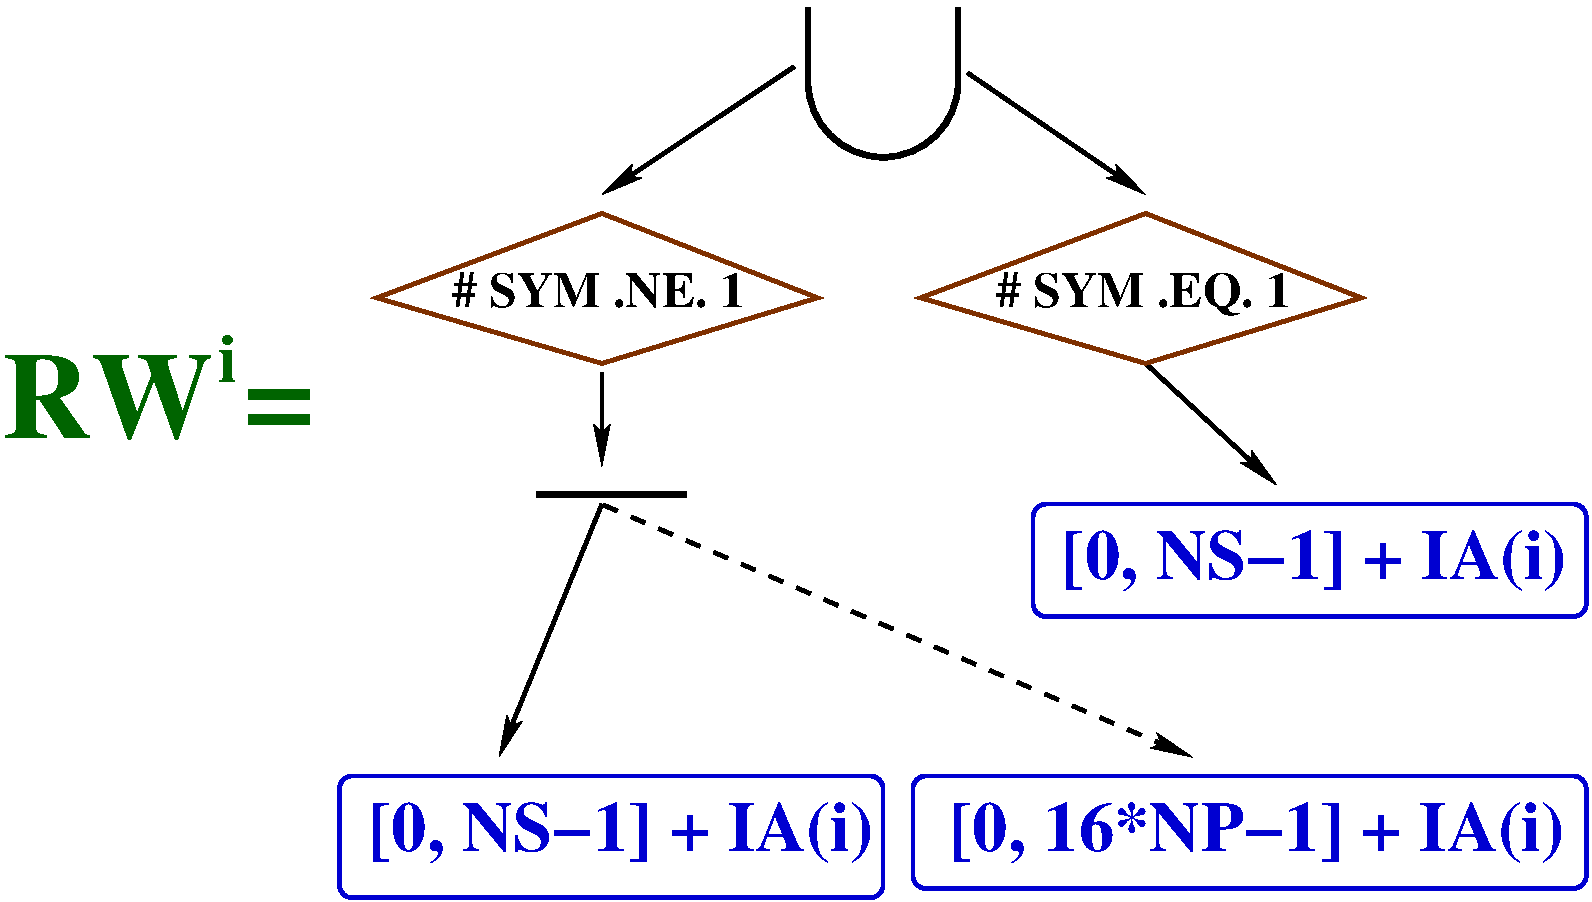
\includegraphics[height=15ex]{Figures/L5-LoopPar/RW_IND_XE}
\end{center}
\end{columns}
\end{block}

\bigskip

In our case, a sufficient condition for {\tt XE} independence is: \bigskip \\ 
$\cup_{i=1}^{N}(RW_i \mbox{ }\cap\mbox{ } (\cup_{k=1}^{i-1}RW_k)) = \emptyset~~~\Leftrightarrow~~~RW_i = \emptyset~~~\Leftrightarrow$

\bigskip

$~~~~~~~~~~~~~~~~~\Leftrightarrow~~~$  
\emph{${\tt SYM}\neq 1\mbox{ }\wedge {\tt NS}\leq 16*{\tt NP}$} 
\end{frame}


\begin{frame}[fragile,t]
  \frametitle{Summary-Based Independence Equations}
\bigskip
Flow and Anti Independence Equation for loop of index \emph{i}:
\begin{equation} \label{FIEq} 
\begin{array}{l r}
S_{find} = \{(\cup_{i=1}^{N} WF_i) \mbox{ }\cap\mbox{ } (\cup_{i=1}^{N} RO_i)\} \mbox{ }\cup & \vspace{1ex} \\ \mbox{ }\mbox{ }\mbox{ }\mbox{ }\mbox{ }\mbox{ }\mbox{ }\mbox{ }\mbox{ }\mbox{ }
\{(\cup_{i=1}^{N} WF_i) \mbox{ }\cap\mbox{ } (\cup_{i=1}^{N} RW_i)\} \mbox{ }\cup & \vspace{1ex} \\ \mbox{ }\mbox{ }\mbox{ }\mbox{ }\mbox{ }\mbox{ }\mbox{ }\mbox{ }\mbox{ }\mbox{ }
\{(\cup_{i=1}^{N}RO_i) \mbox{ }\cap\mbox{ } (\cup_{i=1}^{N}RW_i)\} \mbox{ }\cup  & \vspace{1ex} \\ \mbox{ }\mbox{ }\mbox{ }\mbox{ }\mbox{ }\mbox{ }\mbox{ }\mbox{ }\mbox{ }\mbox{ }
\{ \cup_{i=1}^{N}(RW_i \mbox{ }\cap\mbox{ } (\cup_{k=1}^{i-1}RW_k))\} \mbox{ }\mbox{ }\mbox{ } = \emptyset
\end{array}
\end{equation}

\bigskip

Output Independence Equation for loop of index \emph{i}:
\begin{equation} \label{OIEq} 
\begin{array}{l r}
S_{oind} = \{ \cup_{i=1}^{N}(WF_i \mbox{ }\cap\mbox{ } (\cup_{k=1}^{i-1}WF_k))\} \mbox{ }\mbox{ }\mbox{ } = \emptyset
\end{array}
\end{equation}

\bigskip

Computing $S_{find}$ and $S_{oind}$ solves a more difficult problem than we need, 
i.e., computes the indexes involved in cross-iteration deps. \bigskip

\emp{{\em Loop Independence: when are $S_{find}$ and $S_{oind}$ are empty?}}

\end{frame}


\begin{frame}[fragile,t]
  \frametitle{Key Idea: Predicate-Centric Approach}

\smallskip

{\em Approach centered on extracting arbitrarily-shaped predicates.} 

\bigskip

\begin{block}{Key Idea} 
\begin{columns} 
\column{0.69\textwidth} \vspace{-2ex}
\begin{itemize}
    \item \emp{{\em Source of inaccuracy:}} summary representation not closed under composition w.r.t. set operations. \bigskip
    \item \emph{{\em Language}} representation for summaries ... precise but \emp{expensive} to compute at runtime \bigskip
    \item ``Let's \emph{{\em reason}} about it!'' $\emph{8*NP < NS + 6} \Rightarrow \emp{A - B} = \emptyset \Rightarrow S=\emptyset$!
\end{itemize}
\column{0.33\textwidth} 
\hspace{-2ex}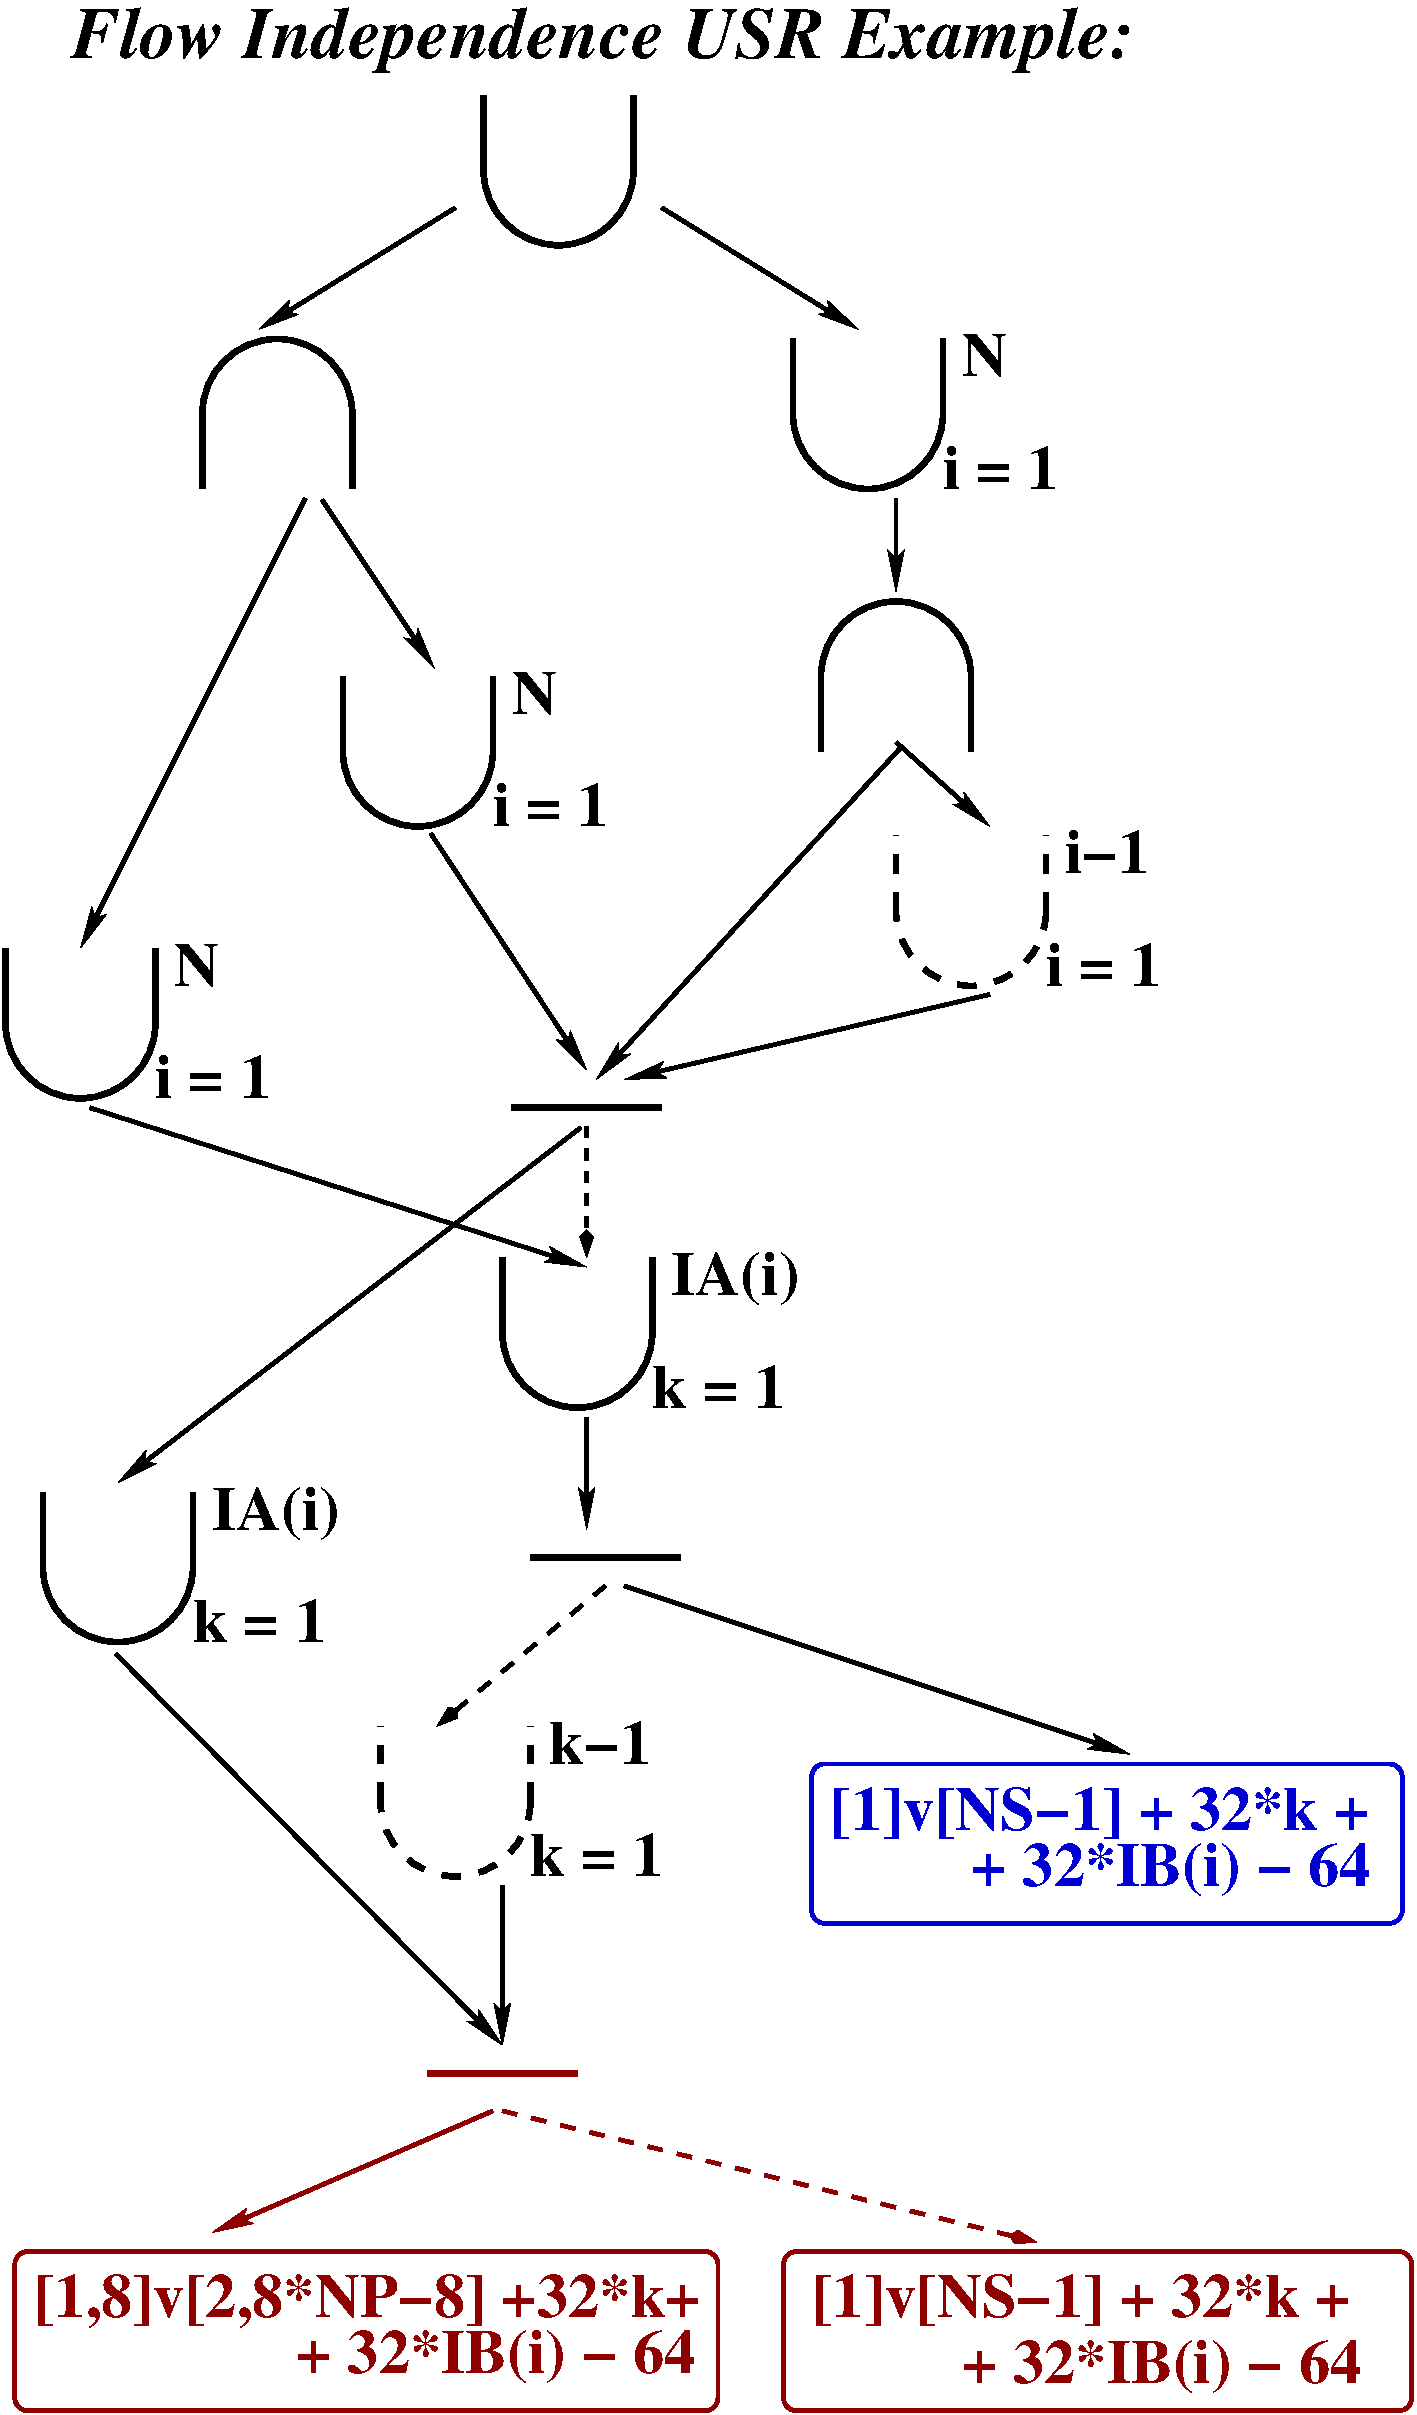
\includegraphics[height=30ex]{Figures/L5-LoopPar/USR_HE_FIND_SOLVH}
\end{columns}
\end{block}

//\alert{Show Calculix from \textsc{Spec2006}}!

\end{frame}


\begin{frame}[fragile,t]
  \frametitle{A Not So Trivial Loop}

\begin{block}{Key Idea} 
\begin{columns} 
\column{0.55\textwidth} 
\begin{colorcode}
k = k0     \emphh{\em Ind.}  k = k0        
DO i=0,N-1 \emphh{\em Var.}  DO i = 0, N-1      
  k = k+2    \emphh{\mymath{\Rightarrow}}    a(k0+2*i)=.. 
  a(k)=..  \emphh{\em Sub.}  ENDDO         
ENDDO            k=k0+MAX(2N-2,0)
   (a)               (b) 
\end{colorcode}
\column{0.33\textwidth} 
\begin{colorcode}
DO i = 0, N-1
 IF(cond(b(i)))THEN 
    civ = civ + 1 \emp{\mymath{\Rightarrow}{\em ?}} 
    a(civ) = ...
ENDIF ENDDO
      (c)
\end{colorcode}

\end{columns}
\end{block}

\begin{itemize}
    \item After induction variable substitution,
            loop (b) is easily found parallel:
          {\tt k0 + 2*i$_1 = $k0 + 2*i$_2 \Rightarrow$ i$_1 = $i$_2$}\pause
    \item Loop (c) is similar to (a) but it is
            more difficult to reason about because
            {\tt civ} cannot be expressed in terms of
            the loop index.
    \item Denote by {\tt civ$_0$}, {\tt civ$_{\mu}^i$}, {\tt civ$_{\gamma}^i$}
            the values of {\tt civ} at the beginning of the loop,
            and at the start and end of iteration {\tt i}.
    \item Express the iteration summary on each path:
        \begin{itemize}
            \item {\tt THEN} branch: {\tt\{civ$_{\mu}^i$+1\}~=~[civ$_{\mu}^i$+1,civ$_{\gamma}^i$]}
            \item {\tt ELSE} branch: {\tt$\emptyset$~=~[civ$_{\mu}^i$+1,civ$_{\gamma}^i$]},
                    (an empty interval has its lower bounds $<$ its upper bound.)
            %\item Hence $W_i = ${\tt [civ$_{\mu}^i$+1,civ$_{\gamma}^i$]}
        \end  {itemize}
\end{itemize}

\end{frame}


\begin{frame}[fragile,t]
  \frametitle{A Not So Trivial Loop}

\begin{block}{Key Idea} 
\begin{columns} 
\column{0.55\textwidth} 
\begin{colorcode}
k = k0     \emphh{\em Ind.}  k = k0        
DO i=0,N-1 \emphh{\em Var.}  DO i = 0, N-1      
  k = k+2    \emphh{\mymath{\Rightarrow}}    a(k0+2*i)=.. 
  a(k)=..  \emphh{\em Sub.}  ENDDO         
ENDDO            k=k0+MAX(2N-2,0)
   (a)               (b) 
\end{colorcode}
\column{0.33\textwidth} 
\begin{colorcode}
DO i = 0, N-1
 IF(cond(b(i)))THEN 
    civ = civ + 1 \emp{\mymath{\Rightarrow}{\em ?}} 
    a(civ) = ...
ENDIF ENDDO
      (c)
\end{colorcode}

\end{columns}
\end{block}

\begin{itemize}
    \item We have deduced that $W_i = ${\tt [civ$_{\mu}^i$+1,civ$_{\gamma}^i$]}

    \item Summarize the accesses of the first $i-1$ iterations:
        \begin{itemize}
            \item {\tt civ$_{\mu}^{i+1} = $civ$_{\gamma}^{i-1}$}
                    since the value of {\tt civ} at the start of an iteration
                    is the same as the one at the end of previous iteration.
            \item $\cup_{k=0}^{i-1} W_k = ${\tt [civ$_{\mu}^0$+1,civ$_{\gamma}^0$]$\cup\ldots\cup$[civ$_{\mu}^{i-1}$+1,civ$_{\gamma}^{i-1}$]} $=$\\{\tt~~~~~~~$=$[civ$_{\mu}^0$+1,civ$_{\gamma}^{i-1}$]$=$[civ$_{\mu}^0$+1,civ$_{\mu}^{i}$]}

        \end  {itemize}

    \item $(\cup_{k=0}^{i-1} W_k) \cap W_i =${\tt[civ$_{\mu}^0$+1,civ$_{\mu}^{i}$]}$\cap${\tt [civ$_{\mu}^i$+1,civ$_{\gamma}^i$]}$= \emptyset$\medskip

    \item We have just proved NO output dependencies occur on array {\tt a}!
\end{itemize}

\end{frame}


\begin{frame}[fragile,t]
  \frametitle{A Not So Trivial Loop}

\begin{block}{Solving the True-Dependence (RAW) on {\tt civ}} 
\begin{columns} 
\column{0.44\textwidth} 
\begin{colorcode}
DO i = 0, N-1
 IF(cond(b(i)))THEN 
    civ = civ + 1 \emp{\mymath{\Rightarrow}{\em ?}} 
    a(civ) = ...
ENDIF ENDDO
\end{colorcode}
\begin{scriptsize}
\begin{itemize}
    \item Extract the loop slice that computes the {\sc civ} value.
            If all accesses to {\tt civ} are in reduction statement
            then compute partial contributions of each iteration.
    \item exclusive scan on the per-iteration contributions give
            the value of {\tt civ} at the beginning of each iteration, and
    \item is plugged in the original loop.
\end{itemize}
\end{scriptsize}
\column{0.52\textwidth} 
\begin{colorcode}
civ0 = civ
DOALL i = 0, N-1
  civ = 0
  IF(cond(b(i))) THEN
    civ = civ + 1
  ENDIF
  civs[i] = civ
ENDDO

civs' = scanExc (+) 0 civs

DOALL i = 0, N-1
  civ = civ0 + civs'[i]
  IF(cond(b(i))) THEN
    civ = civ + 1
    a(civ) = ...
  ENDIF
ENDDO
\end{colorcode}
\end{columns}
\end{block}

\end{frame}

\end{document}

